\documentclass[12pt,a4paper]{report}
\usepackage{graphicx}
\usepackage{amsmath}
\usepackage{fancyhdr}
\usepackage{cite}
\usepackage{framed}
\usepackage{a4wide}
\usepackage{float}
\usepackage{epsfig}
\usepackage{longtable}
\usepackage{enumerate}
\usepackage{afterpage}
\usepackage{multirow}
\usepackage{ragged2e}
\usepackage{gensymb}
\usepackage{amsfonts} 
\usepackage[left=3.5cm,top=1.5cm,right=3cm,bottom=4cm]{geometry}
\usepackage{setspace}           
\usepackage{float}
\usepackage{txfonts}
\usepackage{lipsum}

\newcommand{\Usefont}[1]{\fontfamily{#1}\selectfont}

\usepackage{lscape} % for landscape tables
\renewcommand{\baselinestretch}{1.7} 

\usepackage{blindtext}
\usepackage{xpatch}
\usepackage{url}
\usepackage{leqno}
\usepackage{subcaption}

\linespread{1.5}
\usepackage[intoc, english]{nomencl}
\hyphenpenalty=5000
\tolerance=1000
\usepackage[nottoc]{tocbibind}
\bibliographystyle{IEEEtran}
\renewcommand{\bibname}{References}

%*******************************************************************
%                        Header and Footer   
% This is not required in Technical reports submitted to CET ECE department.
% Please leave it commented                       
%*******************************************************************
%\pagestyle{fancy}
%\fancyhead{}
%\header and footer section
%\renewcommand\headrulewidth{0.1pt}
%\fancyhead[L]{\footnotesize \leftmark}
%\fancyhead[R]{\footnotesize \thepage}
%\renewcommand\headrulewidth{0pt}
%\fancyfoot[R]{\small College of Engineering Trivandrum}
%\renewcommand\footrulewidth{0.1pt}
%\fancyfoot[C]{2020 - 2021}
%\fancyfoot[L]{\small Title of the Seminar/Project}
%*******************************************************************


%*********************Figures*****************************
% Save all figures in the folder figures and include them in your 
% report using the command \includegraphics{figure-name}

\graphicspath{{figures/}}

% figure files can be in jpeg,jpg, png or pdf formats
%*******************************************************************


\begin{document}
	
	
%****The entries in this section are to be filled in by the student with appropriate values *************
% These values are used thoroughout the report 
% please fill in the appropriate values in the brackets {}

\gdef \title{Prison Management System} % Project title
%\gdef \author{Student Name}	 %student name
\gdef \dept{Computer Science and Engineering} %Department
\gdef \degree{Bachelor of Technology} %degree
\gdef \branch{Computer Science and Engineering} %branch
\gdef \college{Model Engineering College} % Name of the College
\gdef \collegeplace{Thrikkakara} % Location of the College
\gdef \studentA{Nihar Niranjan S } %Project batch member 1
\gdef \studentAroll{MDL22CS142} % Project batch member 1 ktu id

\gdef \studentB{Nikith T Rajan } %Project batch member 2
\gdef \studentBroll{MDL22CS147} % Project batch member 2 ktu id

\gdef \studentC{Niranjay Ajayan } %Project batch member 3
\gdef \studentCroll{MDL22CS148} % Project batch member 3 ktu id

\gdef \studentD{Varun Raj R } %Project batch member 4
\gdef \studentDroll{MDL22CS188} % Project batch member 4 ktu id

\gdef \guide{Dr. Sony P} %Project guide
\gdef \guidedes{Assistant Professor}%project guide designation

\gdef \guideco{Prof. Project coguide} %Project coguide
\gdef \guidecodes{Assistant Professor}%project coguide designation

\gdef \guideext{Prof. Project ext guide} %Project external organisation guide
\gdef \guideextdes{Engineer/Scientist}%project external guide designation
\gdef \guideextorg{External guide organization} % Project external guide organization

\gdef \projcordinatorA{Prof. Project coordinator}% Project coordinator 1 
\gdef \projcordinatorAdes{Assistant Professor}% Project coordinator 1 designation

\gdef \projcordinatorB{Prof. Project coordinator 2} % Project coordinator 2 
\gdef \projcordinatorBdes{Assistant Professor}% Seminar coordinator 2 designation

\gdef \hod{Dr. Binu VP} %Head of Department
\gdef \hoddes{Head Of The Department} %HOD designation

\gdef \acadyear{2024 - 25} % Academic year
\gdef \month{November 2024} %Month of Report submission
\gdef \date{08-11-2024} %Date of signing the declaration

%*******************************************************************
% The font pages. The source tex files are there in the folder
%==================================coverpage.tex================================


\newenvironment{coverpage}
\thispagestyle{empty}
\begin{titlepage}
	\begin{center}
		{\Usefont{phv} \Large \bf \title \par}
		\vspace*{40pt}
		\large \em \Usefont{pzc}{ 
			A Project Report \par
			Submitted to the APJ Abdul Kalam Technological University\\
			in partial fulfillment of requirements for the award of degree}\\ [.15\baselineskip] \par
		\Usefont{ppl} {\bfseries  \degree}\\
		in\\
		{\Usefont{ppl} {\bfseries \branch}}\\
		by\\
		\bf {\studentA}(\studentAroll)\\
		\bf {\studentB}(\studentBroll)\\
		\bf {\studentC}(\studentCroll)\\
		\bf {\studentD}(\studentDroll)\\
		\vspace*{40pt}
		\centering
		\begin{figure}[h!]
			\centerline{
\includegraphics[scale=0.4]{figures/meclogo.png}}
		\end{figure}
		
		\vspace{\stretch{0.5}}
		\footnotesize{\bf DEPARTMENT OF COMPUTER SCIENCE AND ENGINEERING} \par
		\bf{GOVT. MODEL ENGINEERING COLLEGE} \par
		\bf{THRIKKAKARA} \par
		\bf{\month}
	\end{center}		
\end{titlepage}	
 %Unless essential Do not edit this tex file


%****************************Mission and vision***************************
% The font pages. The source tex files are there in the folder
%%==================================certificate1.tex================================
% To print name of only the seminar coordinator 1 in the certificate page

\newenvironment{Department Vision and Mission}

	\newpage
  \begin{center}
		
\includegraphics[scale=0.3]{lbslogo.png}	
	\end{center}
	\begin{center}	

		%\vspace{1.5cm}
		\textbf{\large LBS COLLEGE OF ENGINEERING, KASARAGOD\\}	
		\textbf{ \large MULIYAR – 671 542\\} 
            \vspace{0.8cm}
		\textbf{\large DEPT. OF COMPUTER SCIENCE \&  ENGINEERING\\}	
  
	\end{center}
	 \vspace{2cm}
	
	\begin{center}
		\textbf{\underline{\large Vision of Department}}
	\end{center}
 \begin{center}
	To be a renowned centre for education, research, and innovation in the
frontier areas of  {\dept}.
\end{center}
	
	\vspace{1cm}
	
	
	\begin{center}
		\textbf{\underline{\large Mission of Department}}
	\end{center}
 
	\begin{itemize}
  \item Establish and maintain an operational environment to acquire,
impart, create and apply knowledge in Computer Science and
Engineering and inter-disciplinary.
  \item Serve as a resource centre for innovation in design \& development
of hardware and software.
  \item Inculcate leadership qualities, professional ethics and a sense of
social commitment.
\end{itemize}
	
	\thispagestyle{empty}



 %Unless essential Do not edit this tex file



%%********************Certificate*******************

% To print name of only the project coordinator 1 in the certificate page
%==================================certificate1.tex================================
% To print name of only the seminar coordinator 1 in the certificate page

\newenvironment{certificate1}

	\newpage
	\begin{center}	
		%\vspace{1.5cm}
		
		\textbf{DEPT. OF COMPUTER SCIENCE \&  ENGINEERING\\}	
		\textbf{GOVT. MODEL ENGINEERING COLLEGE\\}	
		\textbf{THRIKKAKARA}
		
		\textbf{\acadyear} 
	\end{center}
	
	\begin{center}
		
\includegraphics[scale=0.225]{meclogo.png}	
	\end{center}
	\begin{center}
		\textbf{CERTIFICATE}
	\end{center}
	
	This is to certify that the report entitled \textbf{\title} submitted by \textbf{\studentA}\hspace*{2pt}(\studentAroll), \textbf{\studentB}\hspace*{2pt}(\studentBroll), \textbf{\studentC}\hspace*{2pt}(\studentCroll), and \textbf{\studentD}\hspace*{2pt}(\studentDroll) to the APJ Abdul Kalam Technological University in partial fulfillment of the B.Tech.\ degree in \branch \hspace*{2pt} is a bonafide record of the project work carried out by him under our guidance and supervision. This report in any form has not been submitted to any other University or Institute for any purpose.
	
	
	\begin{singlespace}
    \vspace*{2cm}
    \begin{table}[h!]
        \centering
        \begin{tabular}{p{7cm} p{7cm}} 
            \textbf{\guide} & \textbf{\hod} \\
            (Project Guide) & (Head of Department) \\
            \guidedes & \hoddes \\
            Dept. of CSE & Dept. of CSE \\
            Govt. Model Engineering College & Govt. Model Engineering College \\
            Thrikkakara & Thrikkakara \\
        \end{tabular}
    \end{table}

    \vspace*{1.3cm}
    \end{singlespace}
	
	\thispagestyle{empty} 

% To print names of both the project coordinators in the certificate page
%\include{certificate2} %Please uncomment this and comment the previous line
\pagenumbering{roman} 
%%***************************************************

%==================================acknowledgement.tex=============================
\chapter*{Acknowledgement}%
\addcontentsline{toc}{chapter}{Acknowledgement}%

%\newenvironment{acknowledgement}


\par We take this opportunity to express our deepest sense of gratitude and sincere thanks to everyone who helped us to complete this work successfully. We express our sincere thanks to \hod, Head of Department, \dept, \college\hspace*{2pt} \collegeplace \hspace*{2pt} for providing  us with all the necessary facilities and support.\par

We would like to express our sincere gratitude to the \projcordinatorA, \hspace*{2pt} department of \hspace*{2pt} \dept, \hspace*{2pt} \college \hspace*{2pt} \collegeplace \hspace*{2pt} for the support and co-operation.

We would like to place on record our sincere gratitude to our project guide \guide,\hspace*{2pt}\guidedes,\hspace*{2pt}\dept,\hspace*{2pt}\college \hspace*{2pt} %and our external guide \guideext,\hspace*{2pt}\guideextdes, \hspace*{2pt} \guideextorg   
for the guidance and mentorship throughout this work.

Finally we thank our family, and friends who contributed to the successful fulfillment of this seminar work.

\vspace*{30pt}
\begin{flushright}
	\textbf{\studentA}\\
	\textbf{\studentB}\\
	\textbf{\studentC}\\
	\textbf{\studentD}\\
\end{flushright}
\thispagestyle{plain}

% %==================================declaration.tex================================
%
\newpage
\newenvironment{declaration}
\thispagestyle{empty}
\begin{center}
\vspace*{50pt}
\textbf{DECLARATION}\\
\end{center}
We hereby declare that the project report {\bf{\title}}, submitted for partial fulfillment of the requirements for the award of degree of Bachelor of Technology of the APJ Abdul Kalam Technological University, Kerala is a bonafide work done by us under supervision of \guide \hspace*{2pt} \par
This submission represents our ideas in our own words and where ideas or words of others have been included, we have adequately and accurately cited and referenced the original sources.\par 
We also declare that I have adhered to ethics of academic honesty and integrity and have not misrepresented or fabricated any data or idea or fact or source in my submission. We understand that any violation of the above will be a cause for disciplinary action by the institute and/or the
University and can also evoke penal action from the sources which have thus not been properly cited or from whom proper permission has not been obtained. This report has not been previously formed the basis for the award of any degree, diploma or similar title of any other University.

\noindent \begin{minipage}{0.45\linewidth}
\begin{flushleft}
\vspace{2.5cm}

\collegeplace \\
\date

\end{flushleft} 
\end{minipage}
\hfill
\begin{minipage}{0.45\linewidth}
\begin{flushright}                                      
\vspace{1.5cm}

\textbf{\studentB}\\
% \textbf{\studentB}\\
% \textbf{\studentC}\\
% \textbf{\studentD}\\


\end{flushright} 
\end{minipage}
\thispagestyle{empty}
 %Unless essential Do not edit this tex file



%%****************************Abstract***********************
%============================= abstract.tex================================
\chapter*{Abstract}%
%\addcontentsline{toc}{chapter}{\numberline{}Abstract}%
\addcontentsline{toc}{chapter}{Abstract}%

The Prison Management System (PMS) has been developed to simplify and modernize prison management. The system is meant to replace traditional manual methods of record keeping and administration with a modern digital solution that is secure, accurate and efficient. The PMS enables ease in the management of inmates’ records, monitoring of activities as well as ensuring safety of both inmates and warders.\\

Some of the major aspects about PMS include its ability to facilitate efficient running of jails through its features like adding or removing an inmate from the system, inspecting cell occupancy, assigning rehabilitation jobs among others. Management entails obtaining details about officers on duty and their roles, logging every visitor’s details alongside who they visited, this is because it has powerful search for easily accessible data. It helps streamline operations while improving data accuracy and operational efficiency.\\

Using PMS reduces administrative burden on staff making sure there is more accurate information and smoother operations. It also has reporting tools which assists prison managers in making informed choices. The aim of Prison Management System is therefore directed towards modernizing prison administration, improved data accuracy and enhanced operational efficiency which overall leads into increased safety, effectiveness and correctional facilities performance.\\



\thispagestyle{plain}
%=======================================================================

 % Please type in the abstract in this tex file abstract.tex

%%**********************Table of Contents***********************
\tableofcontents
\listoffigures
\cleardoublepage
\setcounter{page}{1}
\pagenumbering{arabic}



%%********************************Problem Statement***********************
\chapter{Introduction}
\section{Proposed Project}

\subsection{Problem Statement}

The management of prisons is a critical aspect of maintaining order, security, and rehabilitation within correctional facilities. Traditional prison management systems often face challenges in handling large volumes of data, ensuring proper allocation of resources, and maintaining efficiency in operations. Manual tracking of prisoners, staff, tasks, visitors, and incidents can lead to errors, delays, and difficulties in decision-making. Moreover, the lack of integrated and automated solutions makes it difficult to streamline prison operations and ensure smooth coordination between different departments within a facility.\\

\subsection{Proposed Solution}

The Prison Management System aims to address these challenges by providing an automated, digital platform for managing various aspects of prison operations. This system will enable efficient handling of prisoner information, including their personal details, crimes, and status, and will also facilitate the management of staff, visitors, cell allocation, and tasks. The objective is to reduce manual efforts, minimize errors, and provide real-time updates for better decision-making. Furthermore, the system will generate essential reports and allow for easy tracking of incidents, ensuring a higher level of security and accountability.

By integrating all operational aspects into a single system, the Prison Management System will improve efficiency, reduce administrative overhead, and provide an organized and secure environment for both prisoners and staff members.\\


\chapter{System Study Report}
\section{Module Description}

\subsection*{Prisoner Management Module}
\begin{itemize}
    \item \textbf{Description}: The Prisoner Management module ensures that all details regarding prisoners are accurately recorded and easily accessible. This module allows administrators to add new prisoners, update personal and legal information, and remove prisoners when necessary. It is essential for tracking prisoner status, legal cases, and managing overall prison population data.
    \item \textbf{Input}: Prisoner details (name, ID, crime details, sentence information), Updated prisoner details.
    \item \textbf{Output}: Updated prisoner records, deletion of prisoner records.
\end{itemize}

\subsection*{Visitor Management Module}
\begin{itemize}
    \item \textbf{Description}: The Visitor Management module facilitates the tracking and management of visitors coming into the facility. Administrators can register new visitors, link them to specific prisoners, and remove visitor records when required. This ensures that only authorized individuals can visit prisoners, enhancing both security and accountability within the prison.
    \item \textbf{Input}: Visitor details (name, prisoner ID, visit details), Visitor ID.
    \item \textbf{Output}: Updated visitor records, deletion of visitor records.
\end{itemize}

\subsection*{Cell Management Module}
\begin{itemize}
    \item \textbf{Description}: The Cell Management module is responsible for overseeing the allocation and management of prison cells. It allows administrators to add new cells to the system, delete unused or obsolete cells, and reallocate prisoners between cells to maintain safety, security, and optimal prison operations. This ensures a well-organized facility and efficient use of resources.
    \item \textbf{Input}: Cell details (Cell ID, Cell Location), Prisoner ID, Reallocation details.
    \item \textbf{Output}: Updated cell and prisoner allocation.
\end{itemize}

\subsection*{Staff Management Module}
\begin{itemize}
    \item \textbf{Description}: The Staff Management module enables the efficient handling of prison staff records. Administrators can register new staff members, remove staff when necessary, and manage user access for various staff roles. By ensuring that staff have the appropriate permissions, this module helps maintain secure and effective prison operations.
    \item \textbf{Input}: Staff details (name, role, contact details), User ID.
    \item \textbf{Output}: Updated staff records, user access management.
\end{itemize}

\subsection*{Crime Management Module}
\begin{itemize}
    \item \textbf{Description}: The Crime Management module is used to manage and update the criminal records of prisoners. It allows administrators to add crime details related to each prisoner, update existing crime information, or remove outdated records. This ensures accurate tracking of prisoner histories and supports legal proceedings within the correctional facility.
    \item \textbf{Input}: Crime details (crime type, date, prisoner ID), Updated crime information.
    \item \textbf{Output}: Updated crime records, removal of crime details.
\end{itemize}

\subsection*{Job Management Module}
\begin{itemize}
    \item \textbf{Description}: The Job Management module allows for the efficient assignment and management of tasks given to prisoners. Administrators can add job details, update existing tasks, and remove completed or redundant job assignments. This module helps track the work done by prisoners, contributing to their rehabilitation and prison maintenance efforts.
    \item \textbf{Input}: Job details (task description, prisoner ID, job assignment), Updated job details.
    \item \textbf{Output}: Updated prisoner job assignments, removal of job records.
\end{itemize}

\subsection*{Work Management Module}
\begin{itemize}
    \item \textbf{Description}: The Work Management module tracks the work done by prisoners within the facility. It allows administrators to record details of tasks or jobs completed by prisoners, including work hours, and ensures proper documentation of all work activities. The module also enables the calculation of total work hours logged by each prisoner for monitoring productivity and compliance.
    \item \textbf{Input}: Work details (task completed, prisoner ID, work hours), Updated work details.
    \item \textbf{Output}: Updated work records, total work hours for prisoners.
\end{itemize}
\section{Technological Stacks}

\subsection*{React (Frontend)}

\subsubsection{Description}
React is an open-source JavaScript library for building user interfaces, particularly single-page applications where dynamic data is frequently updated and displayed.

\subsubsection{Role in Project}
React will be used to create the user interface for the "Prison Management" system. It will handle user interactions and update the UI based on user inputs, ensuring a dynamic and responsive experience.

\subsection*{Python Flask (Backend)}

\subsubsection{Description}
Flask is a lightweight, open-source web framework for Python, designed to make it easy to build web applications.

\subsubsection{Role in Project}
Flask will serve as the backend, acting as a gateway between the user interface and the database. It will handle communication with the database through various functions, ensuring smooth data retrieval and manipulation.

\subsection*{MySQL (Database)}

\subsubsection{Description}
MySQL is a popular open-source Relational Database Management System (RDBMS) that uses SQL (Structured Query Language) for database operations.

\subsubsection{Role in Project}
MySQL will store all the data, which includes details like the list of crimes, prisoner details, staff details, user logins, cell allocations, visitor details, and work assigned to each prisoner.

\subsection*{hashlib (Backend)}

\subsubsection{Description}
The \texttt{hashlib} module implements a common interface for many secure cryptographic hash and message digest algorithms. There is one constructor method for each type of hash, and all return a hash object with the same simple interface.

\subsubsection{Role in Project}
\texttt{hashlib} will be used to ensure data integrity by generating hash values and encrypting the data. This is particularly useful for storing sensitive information like passwords and ensuring that data is not tampered with.
\section{Constraints}

\subsection*{Data Security and Privacy}
\textbf{Description:} Ensuring the security and privacy of sensitive data, such as prisoner details, staff information, and visitor logs, is a top priority. This involves implementing strong encryption techniques, secure authentication mechanisms, and access controls to prevent unauthorized access.

\subsection*{System Availability}
\textbf{Description:} The Prison Management System must ensure high availability, meaning the system should be accessible and operational at all times, with minimal downtime. This includes planning for disaster recovery and failover mechanisms.

\subsection*{Performance and Scalability}
\textbf{Description:} The system should be able to handle large amounts of data and simultaneous user requests, particularly during peak times such as prisoner intake, staff updates, or visitor records.

\subsection*{Usability}
\textbf{Description:} The Prison Management System must be user-friendly, with intuitive interfaces that reduce the complexity for staff members, prison officers, and administrators.

\subsection*{Regulatory Compliance}
\textbf{Description:} The system must comply with all relevant regulations, laws, and standards concerning the management of prisons and correctional facilities. This includes adherence to privacy laws, data protection regulations (e.g., GDPR), and local prison system protocols.

\subsection*{Integration with External Systems}
\textbf{Description:} The system may need to integrate with other existing systems within the prison or external entities such as law enforcement agencies or rehabilitation centers. This integration must be seamless and secure.

\subsection*{Cost and Budget Constraints}
\textbf{Description:} The project must be developed and maintained within the allocated budget. This constraint affects the choice of technologies, development tools, and hosting infrastructure.

\subsection*{User Training and Adoption}
\textbf{Description:} The system must be easy for users to learn and adopt. This includes ensuring that staff members are trained and comfortable using the system within a short period of time.

\section{Operating System}
The system operates in a web-based environment, ensuring accessibility across various devices and platforms. It is compatible with standard web browsers and requires a stable internet connection for optimal functionality.

\section{User Documentation}
 All documentation will be made in accordance with requirements pertaining to open source software
 under the GNU General Purpose License. Online documentation will be available within the website
 to determine proper use.

 \section{Assumptions and Dependencies}
 
 \begin{itemize}
     \item The system assumes that handwritten answers are legible and follow standard conventions.
     \item We also assume that the user has a consistent internet connection for seamless operation.
     \item The system relies on the availability of a well-defined answer key against which student responses are evaluated.
 \end{itemize}

\chapter{Project Design}
\section{High Level Design}
\subsection{Database Design}
    The database consists of 9 tables as described in the following ER diagram. The Prisoner table contains basic details about the the current conviction of the prisoner and the Prisoner Details table contains more descriptive details. The Work table contains details of the community service done by the prisoners. The Visitor Details table contains details of visitors visiting the various prisoners. The Cells table contains details regarding the occupants of each cell. The Staff and Login Details tables contains staff details and their login credentials respectively. The password is stored in a hashed form to enhance security.
    \begin{figure}[H]
        \centering
        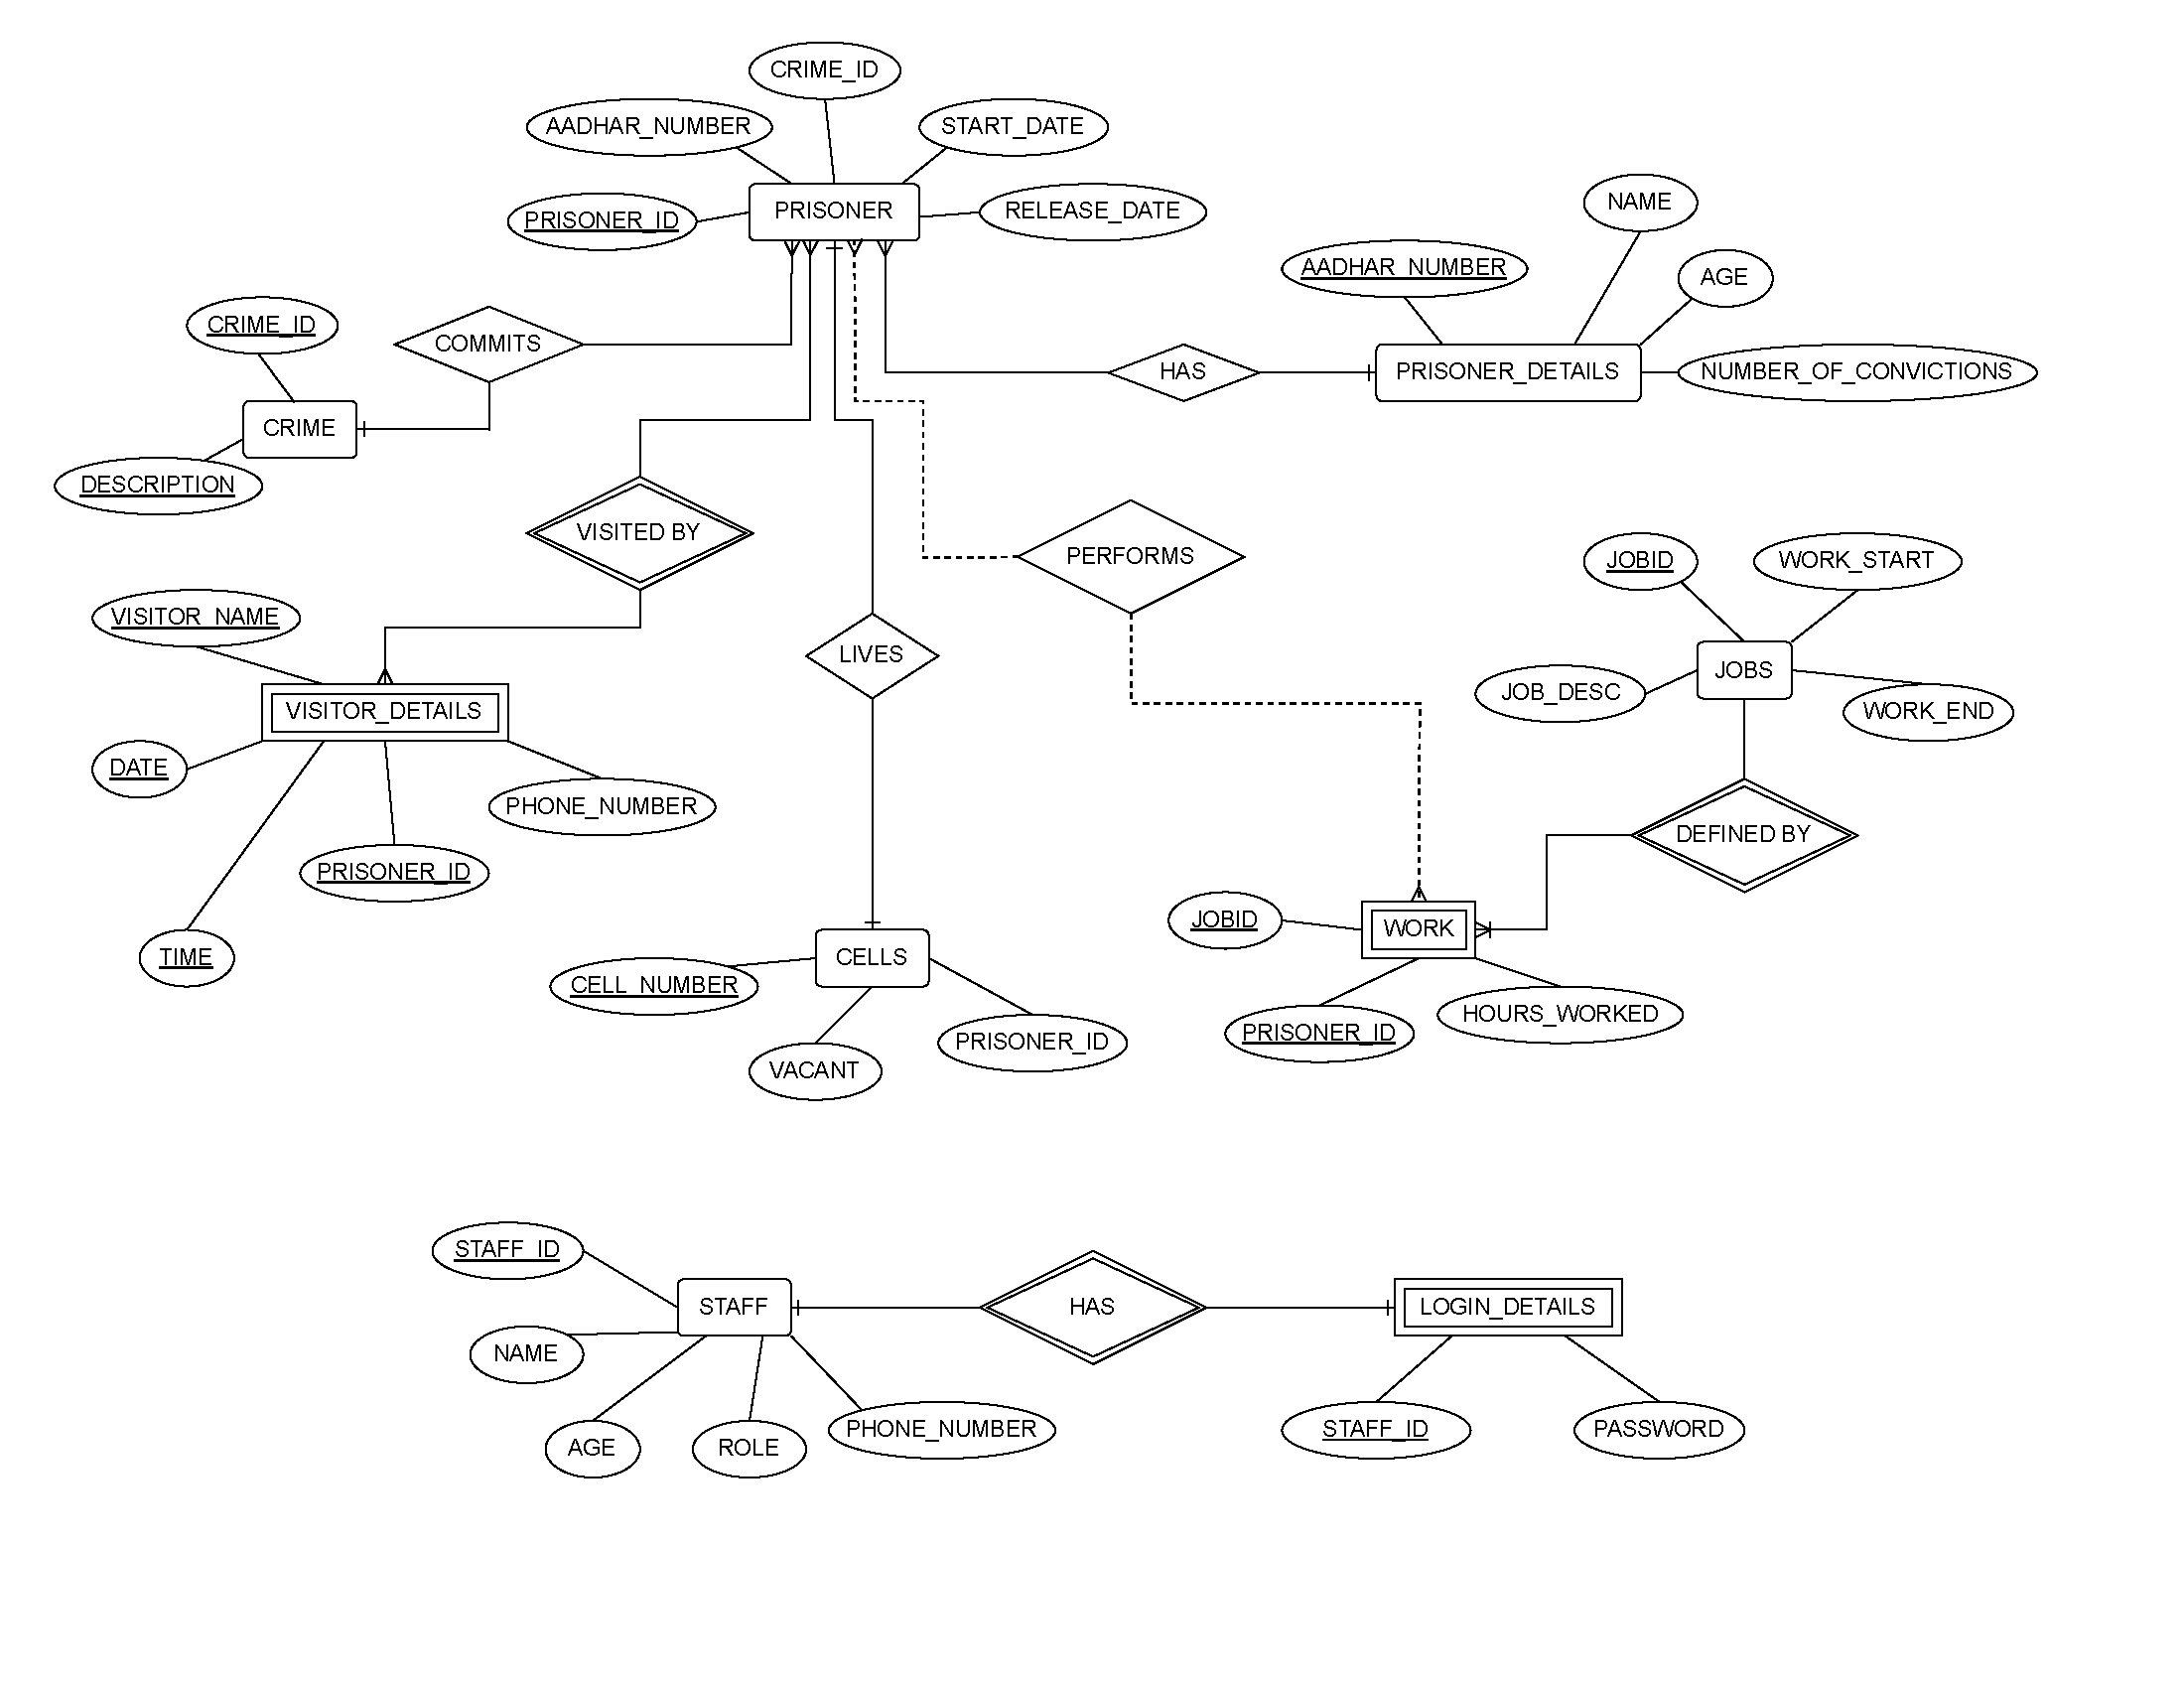
\includegraphics[ height=0.54\textheight]{er.png}
        \caption{ER Diagram}
        \label{fig:er}
    \end{figure}
\newpage
\subsection{System Design}
    The following use-case diagram is a graphical depiction of a user's possible interactions with a system. 
    \begin{figure}[H]
        \centering
        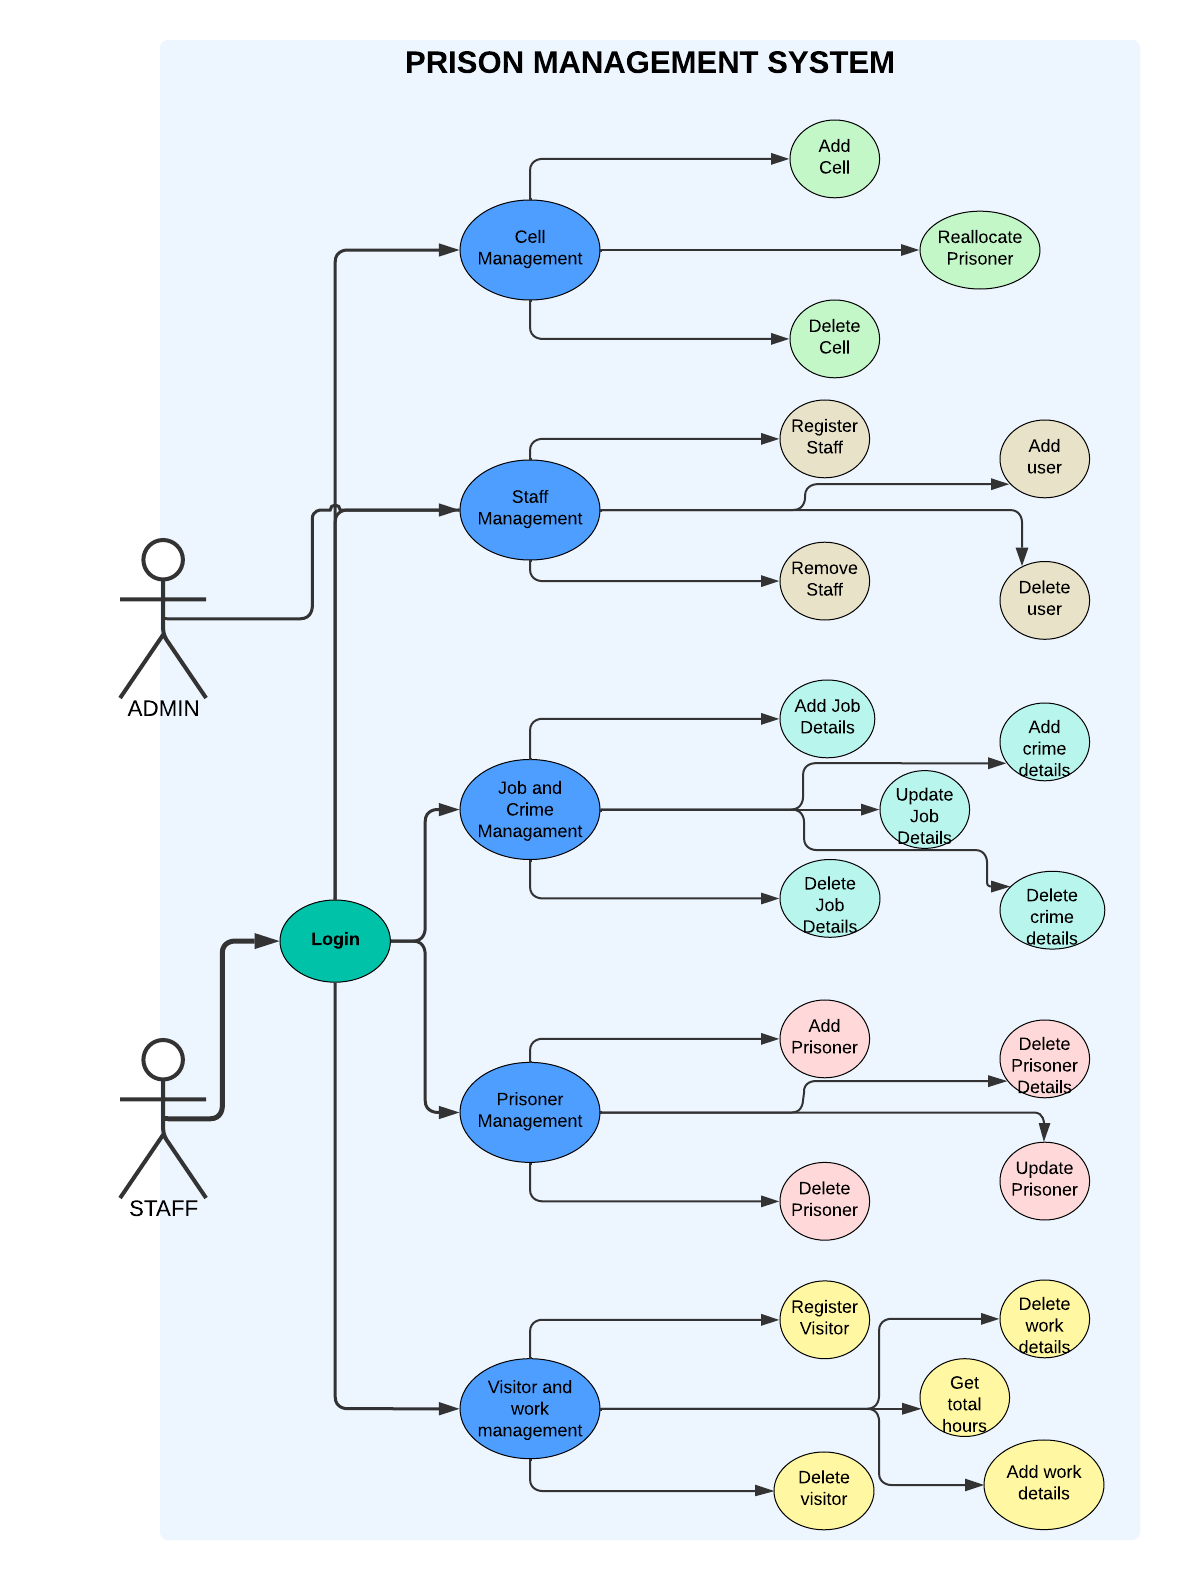
\includegraphics[width=\textwidth]{figures/use-case.png}
        \caption{Use-Case Diagram}
        \label{fig:usecase}
    \end{figure}
    \newpage
    The following class diagram shows the modularization of the system into different components. Different objects are created in order to interface with the database.
    \begin{figure}[H]
        \centering
        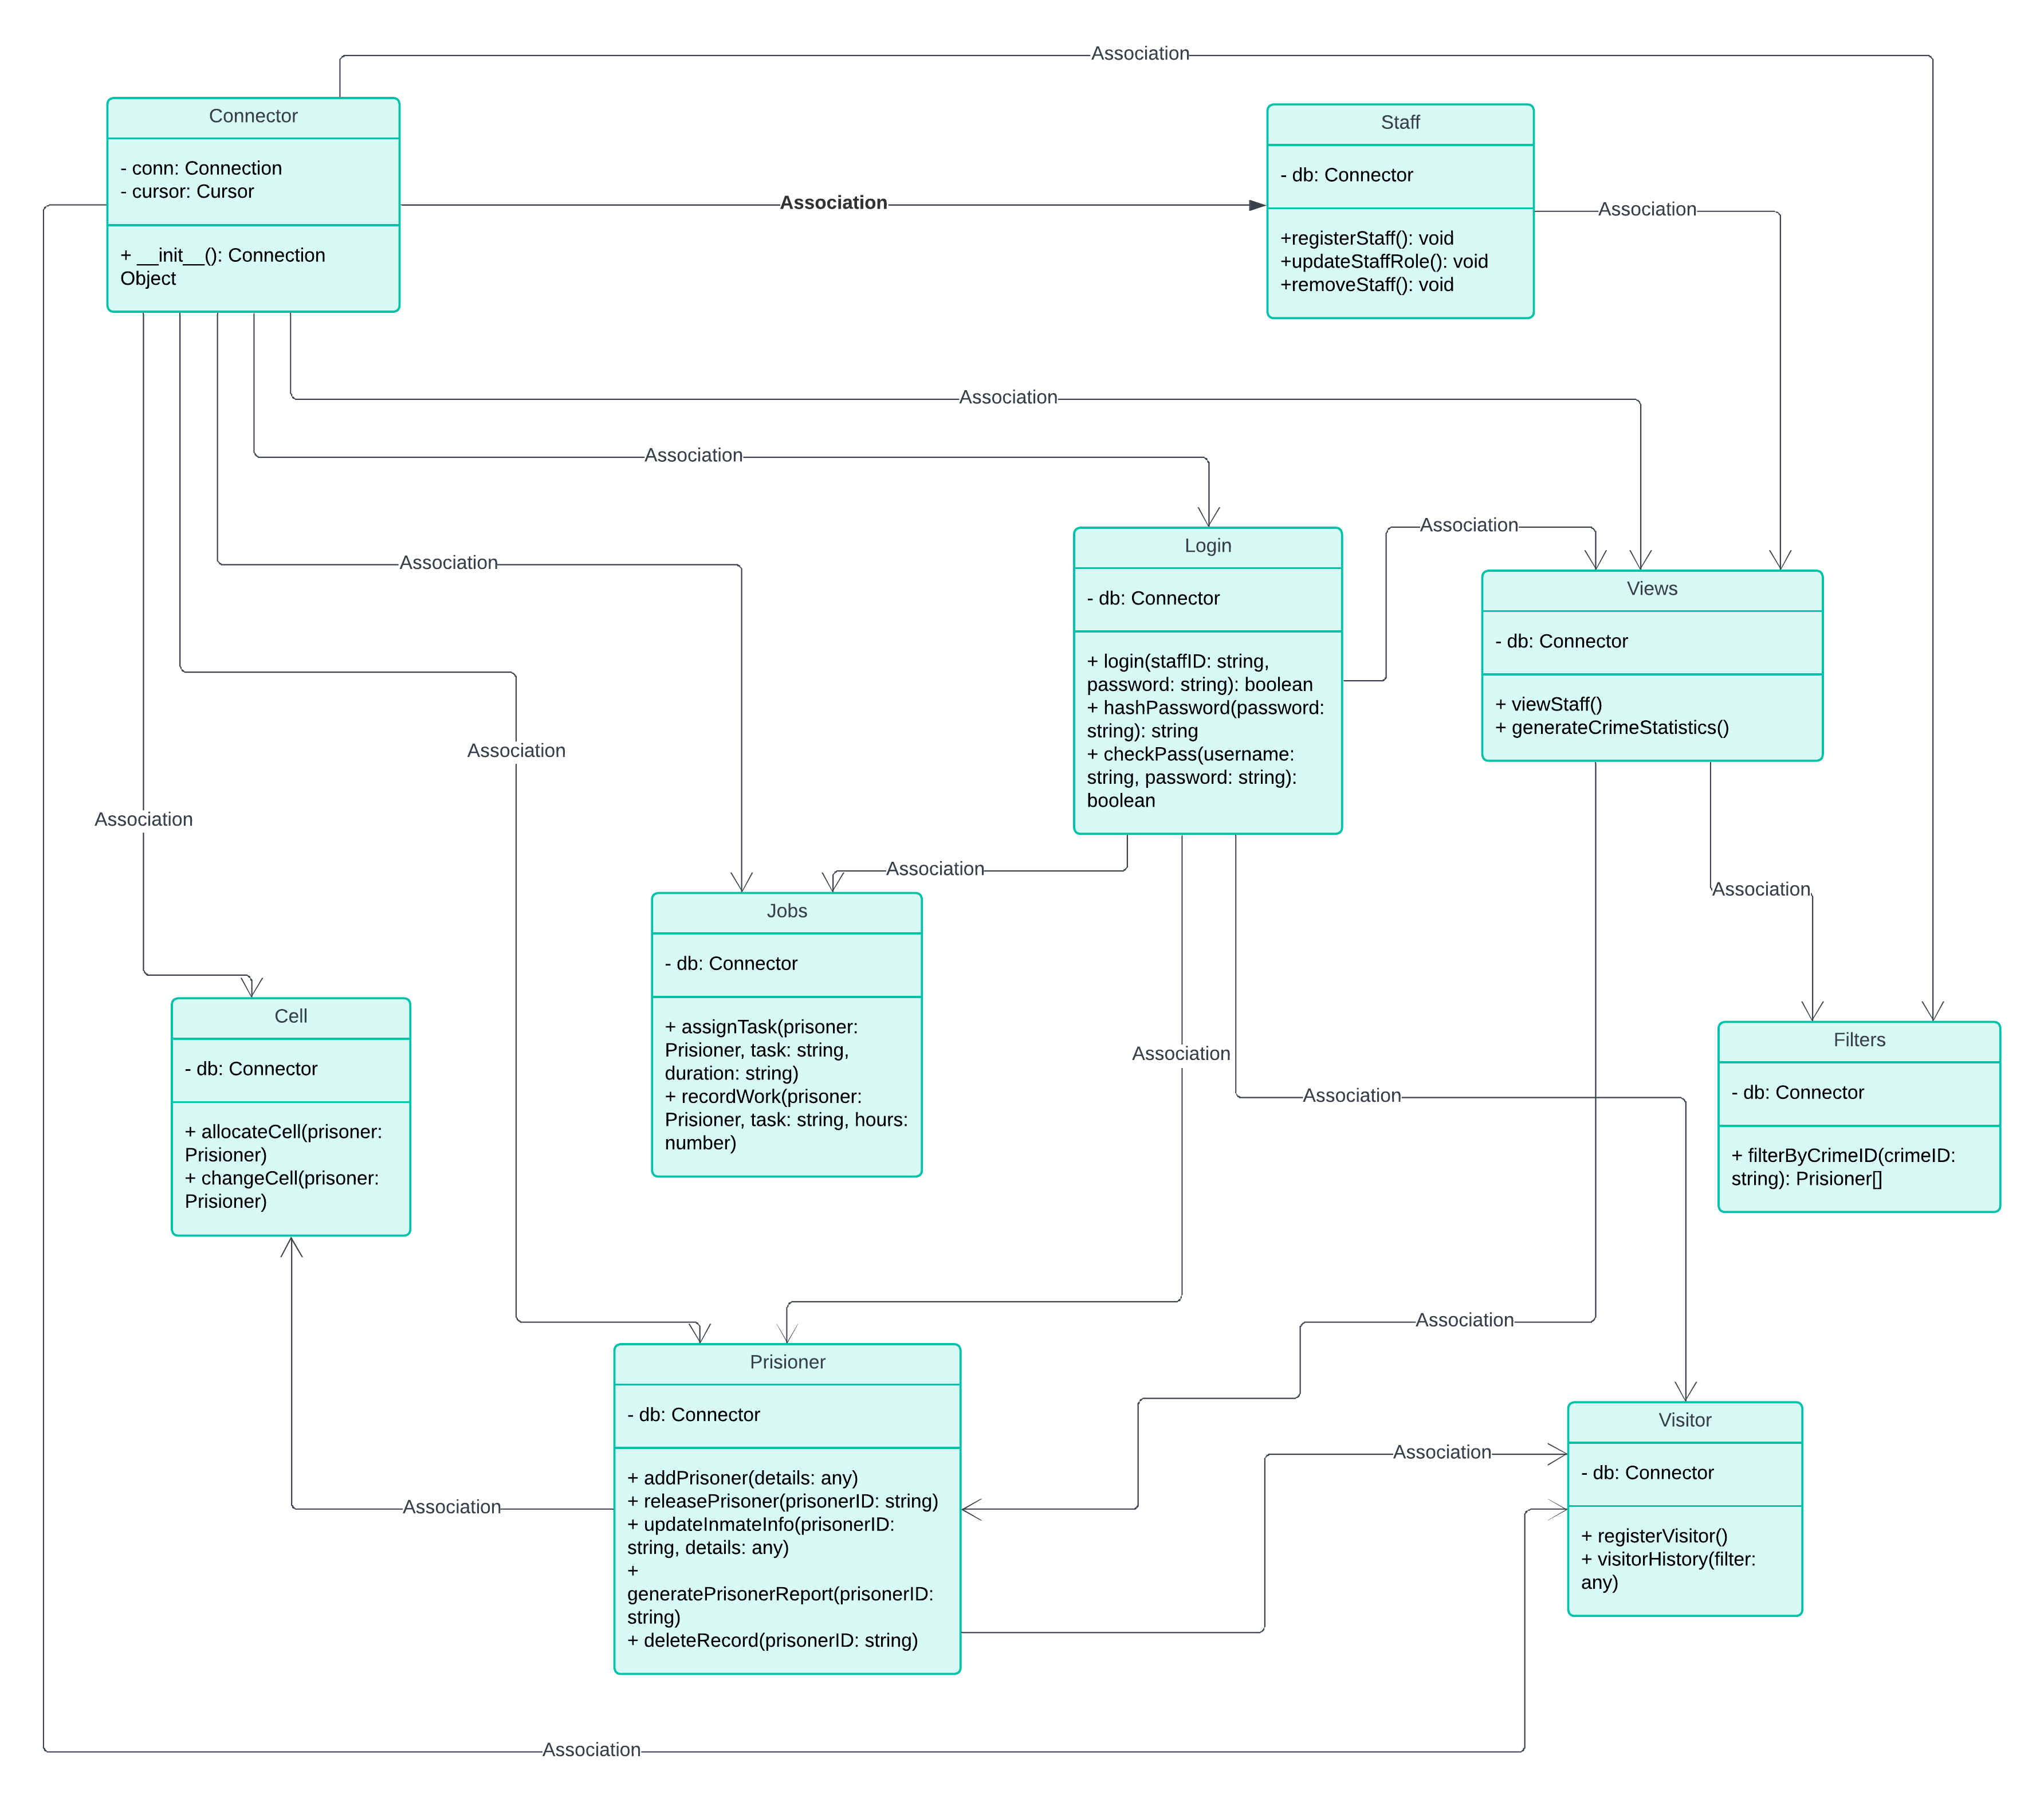
\includegraphics[angle=90, width=\textwidth, height=\textheight, keepaspectratio]{class3.png}
        \caption{Class Diagram}
        \label{fig:class}
    \end{figure}
    \newpage
    The following sequence diagram shows the sequence of operation of the system when a user interacts with it. The warden can use the various modules to manage different aspects of the prison such as staff and prisoner management.
    \begin{figure}[H]
        \centering
        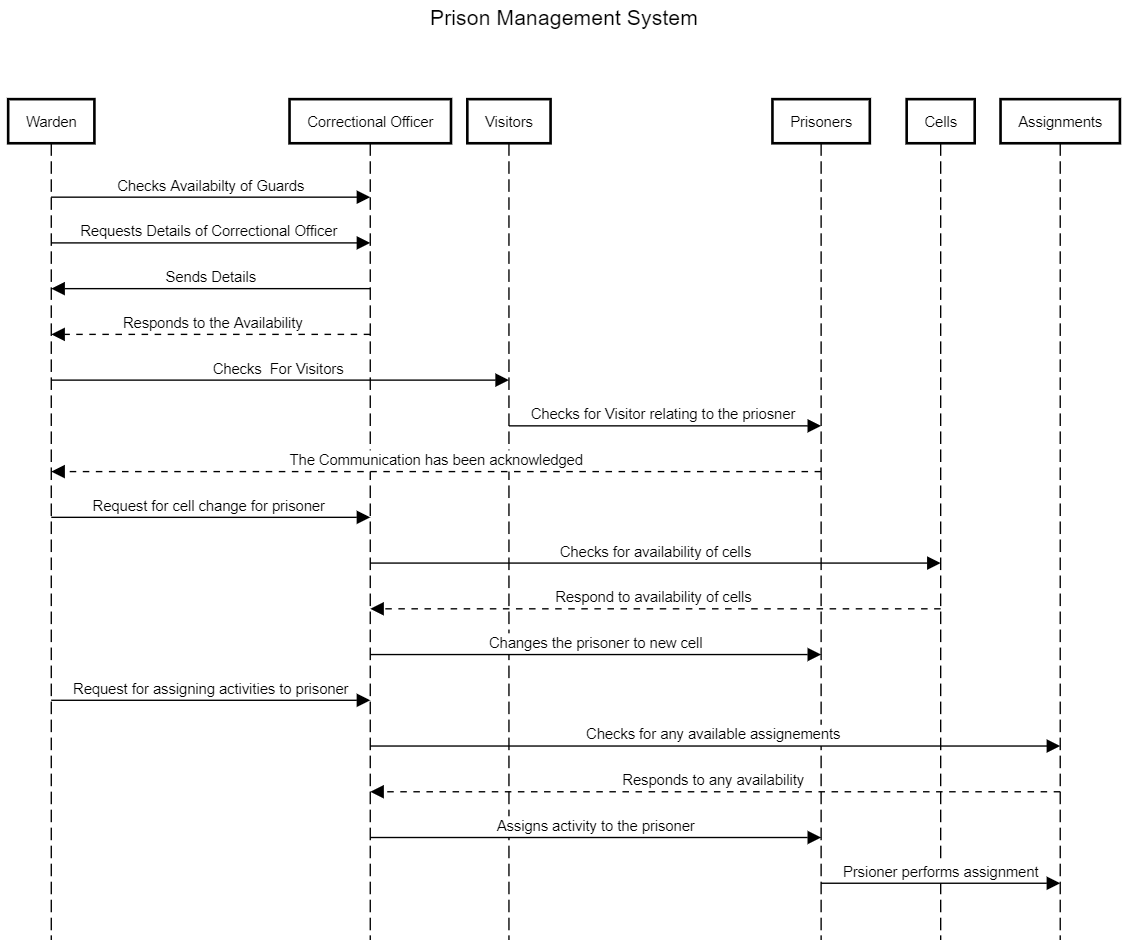
\includegraphics[scale=0.45, width=\textwidth]{sequence.png}
        \caption{Sequence Diagram}
        \label{fig:sequence}
    \end{figure}
    The Activity Diagram for the  PMS visually represents the flow of activities and actions within the system. It starts with the user arriving at the home page where they can log in. After providing correct credentials, the user is logged in and redirected to the dashboard where they can perform various actions related to the PMS. The user can view details regarding the prisoners, visitors, community service, cells, and staff and can add, remove, and modify the various details.
    \begin{figure}[H]
        \centering
        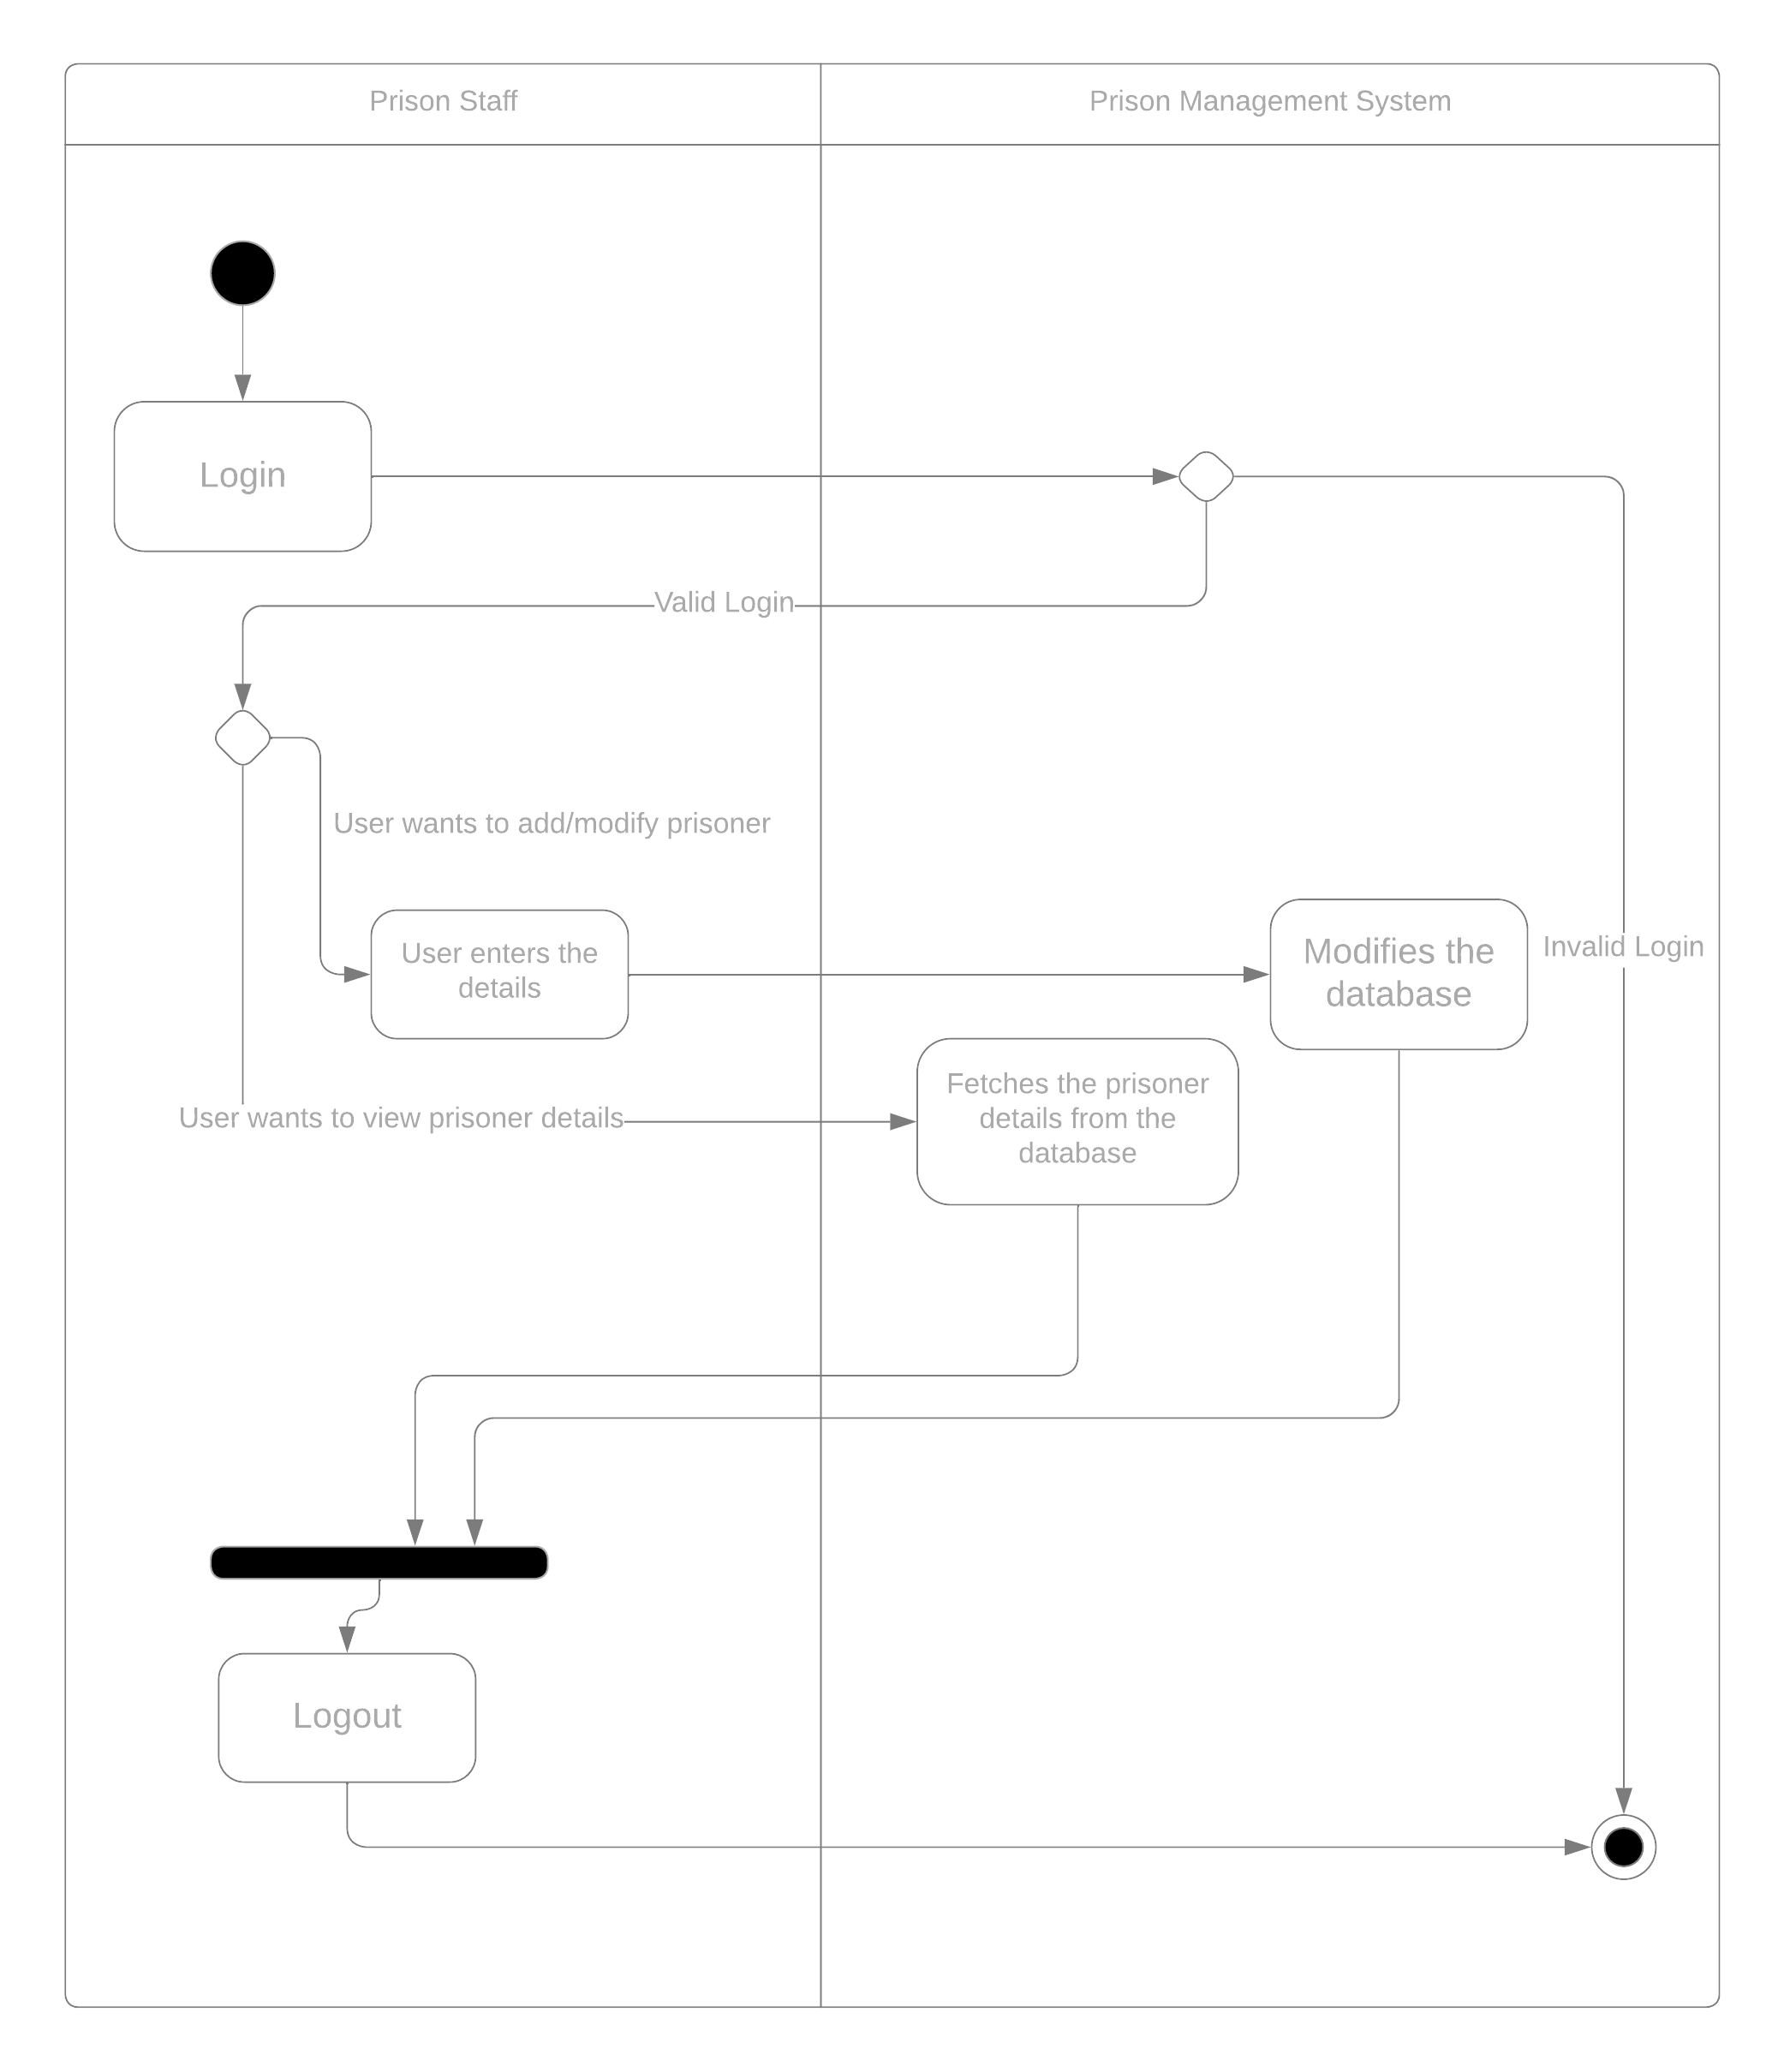
\includegraphics[scale=0.4, width=\textwidth]{activity.png}
        \caption{Activity Diagram}
        \label{fig:activity}
    \end{figure}
\subsection{User Interface}
    When the user opens the website, the landing page shows a form to login to the PMS. On successful login, the users are redirected to the dashboard. Here, they have the provision to view and modify various details regarding the prison. Upon choosing an option, they are shown the values in the table, along with buttons to add, delete or modify the various details.
    
\section{Hardware and Software Requirements}
\subsection{Hardware Requirements}
\begin{enumerate}
    \item Operating System: Windows 7 and above, Linux and macOS.
    \item Processor: 2 GHz processor or better.
    \item RAM: Minimum 4 GB RAM.
    \item Hard disk: Minimum 1 GB HDD Space.
    \item Internet Connection: Minimum 1 Mbps bandwidth.
\end{enumerate}    
\subsection{Software Requirements}
\begin{enumerate}
    \item \textbf{Programming Languages:} Python is used due to its extensive libraries and frameworks. JavaScript is used to create the Frontend using the ReactJS framework \cite{reactdocs}.

    \item \textbf{Libraries and Packages:} Hashlib is used to hash the passwords and MySQL Connector is used to connect with the database.
    
    \item \textbf{Integrated Development Environment (IDE):} IDE for coding, debugging, and testing. Common choices include Jupyter Notebooks, Visual Studio Code, or PyCharm.

    \item \textbf{Database Management System (DBMS):} To store and manage the grading data. MySQL is a popular relational database that was used for this project.
    
    \item \textbf{Web Framework:} Web Framework Flask \cite{flaskdocs} was used for Backend development.
    
    \item \textbf{Version Control:} Implement version control using Git to track changes in your codebase and collaborate with others.
\end{enumerate}


\chapter{Testing}

\subsection{Unit Testing}
\begin{itemize}
    \item \textbf{Cell Management Module}: Verify the correct addition, deletion, and reallocation of cells and prisoner placements within the database.
    \item \textbf{Staff Management Module}: Ensure accurate registration, removal of staff, and management of user access rights.
    \item \textbf{Job Management Module}: Test the functionality of adding, updating, and deleting prisoner job assignments.
    \item \textbf{Crime Management Module}: Validate the addition, modification, and removal of crime details associated with prisoners.
    \item \textbf{Prisoner Management Module}: Confirm accurate addition, updating, and deletion of prisoner records in the system.
    \item \textbf{Visitor Management Module}: Verify registration and deletion of visitor records, ensuring they link accurately to prisoners.
    \item \textbf{Work Management Module}: Ensure correct recording of work details, removal of work records, and calculation of total work hours for prisoners.
\end{itemize}

\subsection{Integration Testing}
\begin{itemize}
    \item \textbf{Prison Management System Integration}: Assess the collective performance of Cell, Staff, Job, Crime, Prisoner, Visitor, and Work Management modules to ensure they work together seamlessly.
\end{itemize}

\subsection{System Testing}
\begin{itemize}
    \item \textbf{End-to-End Functionality}: Test end-to-end functionality to ensure the system meets all requirements for prisoner management, cell allocation, staff operations, and work logging.
\end{itemize}

\subsection{User Acceptance Testing (UAT)}
\begin{itemize}
    \item \textbf{Administrative Tasks}: Evaluate the usability of the system by having administrators perform tasks like adding prisoners, reallocating cells, and managing job details.
\end{itemize}

\subsection{Security Testing}
\begin{itemize}
    \item \textbf{User Authentication Measures}: Examine the authentication system for vulnerabilities, ensuring only authorized access.
    \item \textbf{Data Encryption}: Validate the encryption of sensitive prisoner and staff data within the system.
    \item \textbf{Access Control}: Confirm the access control mechanisms to prevent unauthorized actions and data breaches.
\end{itemize}

\subsection{Performance Testing}
\begin{itemize}
    \item \textbf{Concurrent User Actions}: Assess system performance when handling multiple concurrent tasks, such as adding prisoners, reallocating cells, or updating job details.
\end{itemize}

\subsection{Regression Testing}
\begin{itemize}
    \item \textbf{Impact of Changes}: Ensure modifications to the Cell, Staff, or other modules do not affect existing functionalities in unintended ways.
\end{itemize}

\subsection{User Interface (UI) Testing}
\begin{itemize}
    \item \textbf{Consistency and Responsiveness}: Review UI elements for visual consistency and responsiveness across different screens and user roles.
\end{itemize}

\subsection{Error Handling Testing}
\begin{itemize}
    \item \textbf{Error-Triggering Scenarios}: Subject the system to various error-prone scenarios (e.g., invalid data inputs or network failures) to ensure proper error messages and handling.
\end{itemize}

\subsection{Load Testing}
\begin{itemize}
    \item \textbf{System Capacity}: Test the system's ability to handle a high volume of prisoner records, visitor registrations, and staff actions simultaneously.
\end{itemize}

\subsection{Compatibility Testing}
\begin{itemize}
    \item \textbf{Cross-Browser and Cross-Device Compatibility}: Ensure that the system functions correctly across different browsers and devices used by staff.
\end{itemize}

\subsection{Usability Testing}
\begin{itemize}
    \item \textbf{User Experience Evaluation}: Collect feedback on the ease of use, intuitiveness, and efficiency of the system to identify areas for improvement.
\end{itemize}


\chapter{Screenshots}%
%\addcontentsline{toc}{chapter}{\numberline{}Abstract}%
%\addcontentsline{toc}{chapter}{Screenshots}%
    \begin{figure}[H]
        \centering
        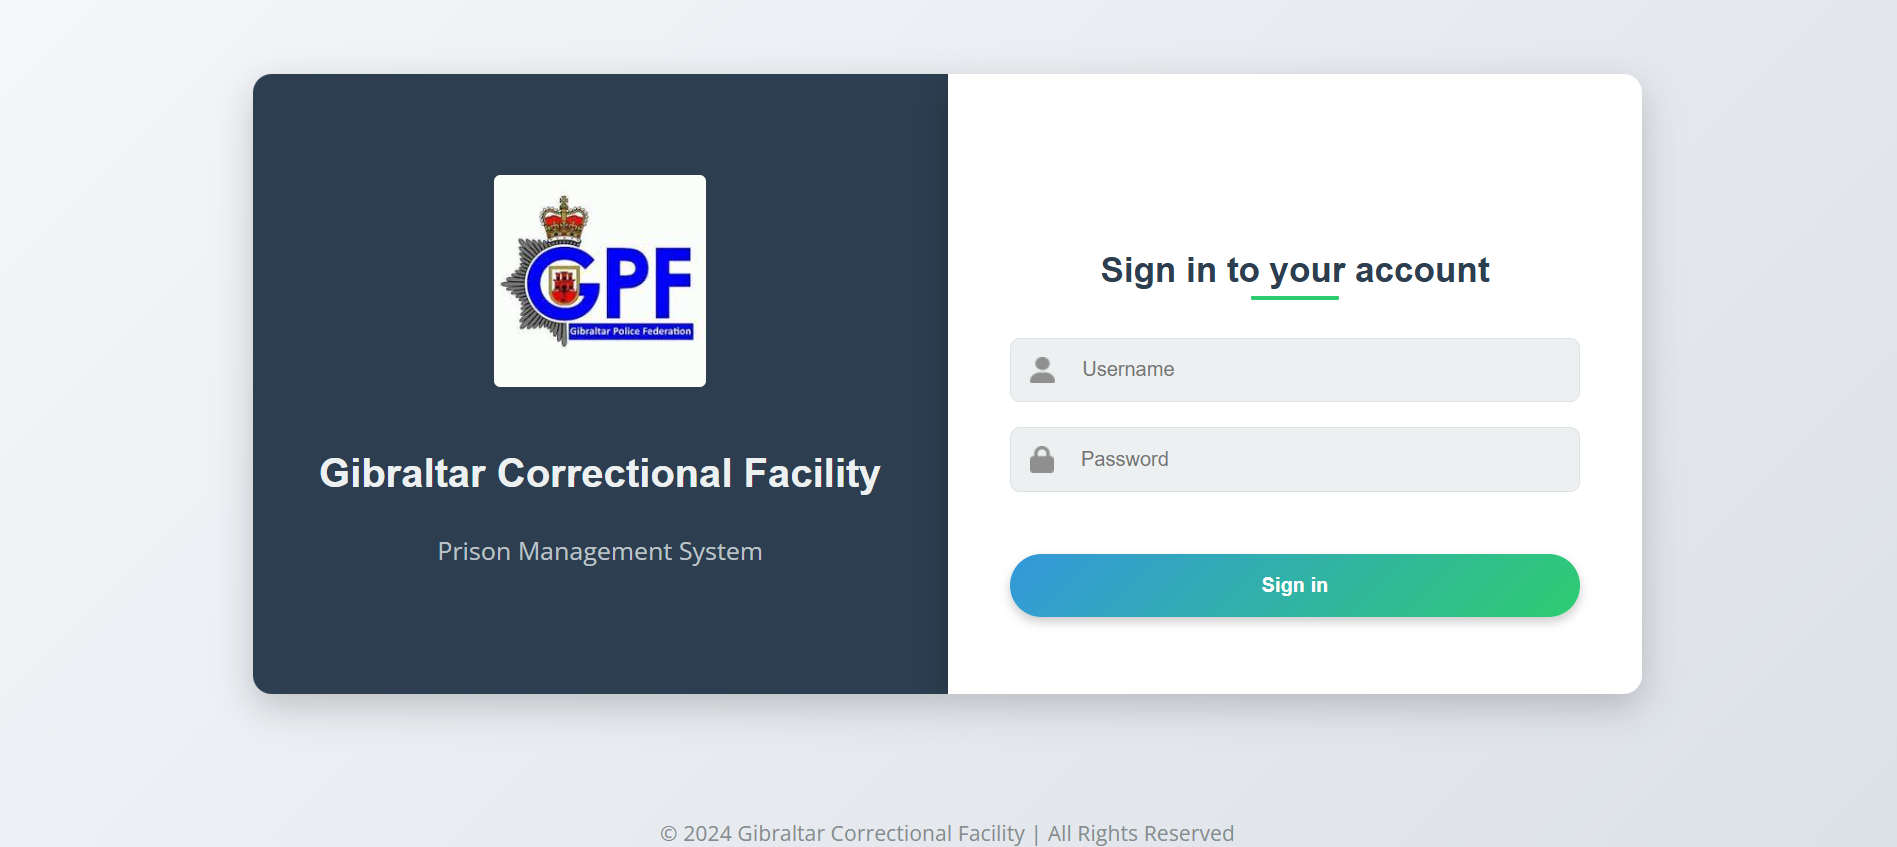
\includegraphics[width=0.8\textwidth]{screenshots/login.png}
        \caption{Login Screen}
        \label{fig:login}
    \end{figure}
    \begin{figure}[H]
        \centering
        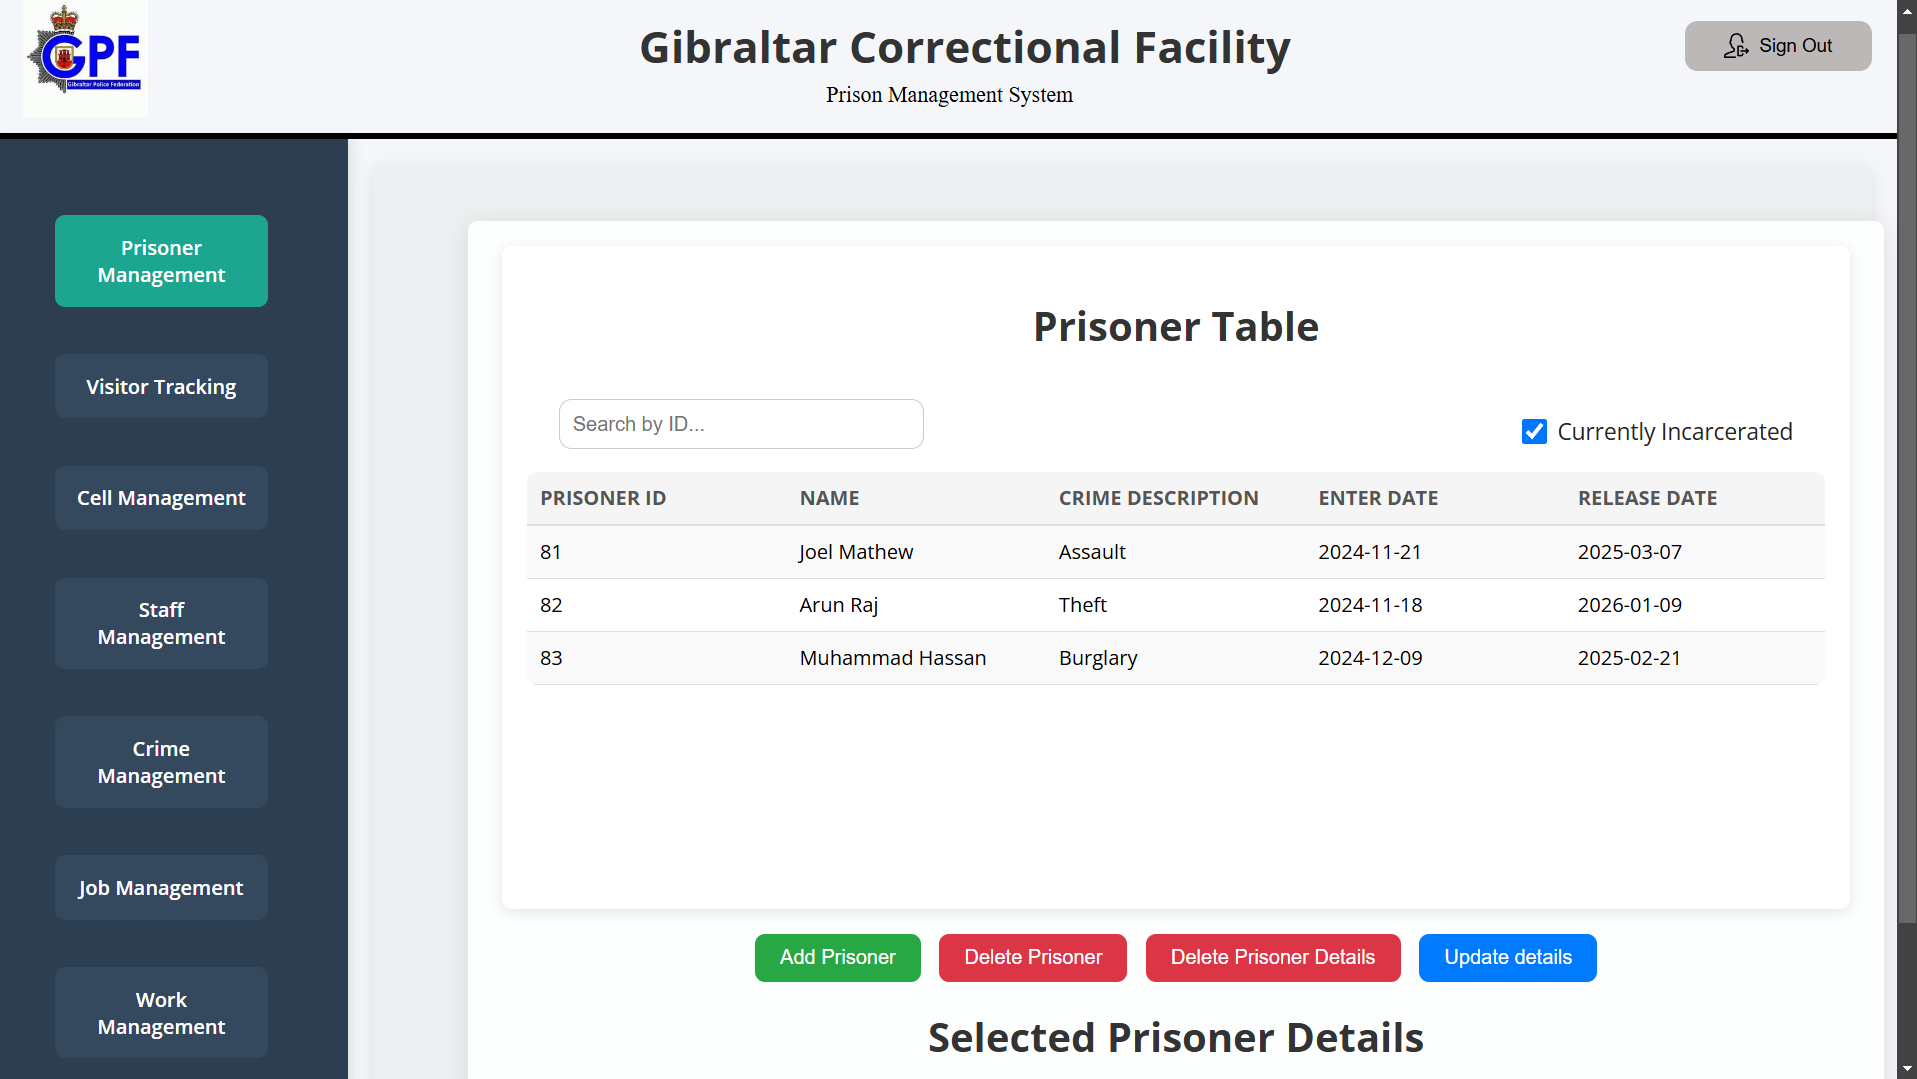
\includegraphics[width=0.8\textwidth]{screenshots/prisoner.png}
        \caption{List of Prisoners}
        \label{fig:prisoner}
    \end{figure}
    \begin{figure}[H]
        \centering
        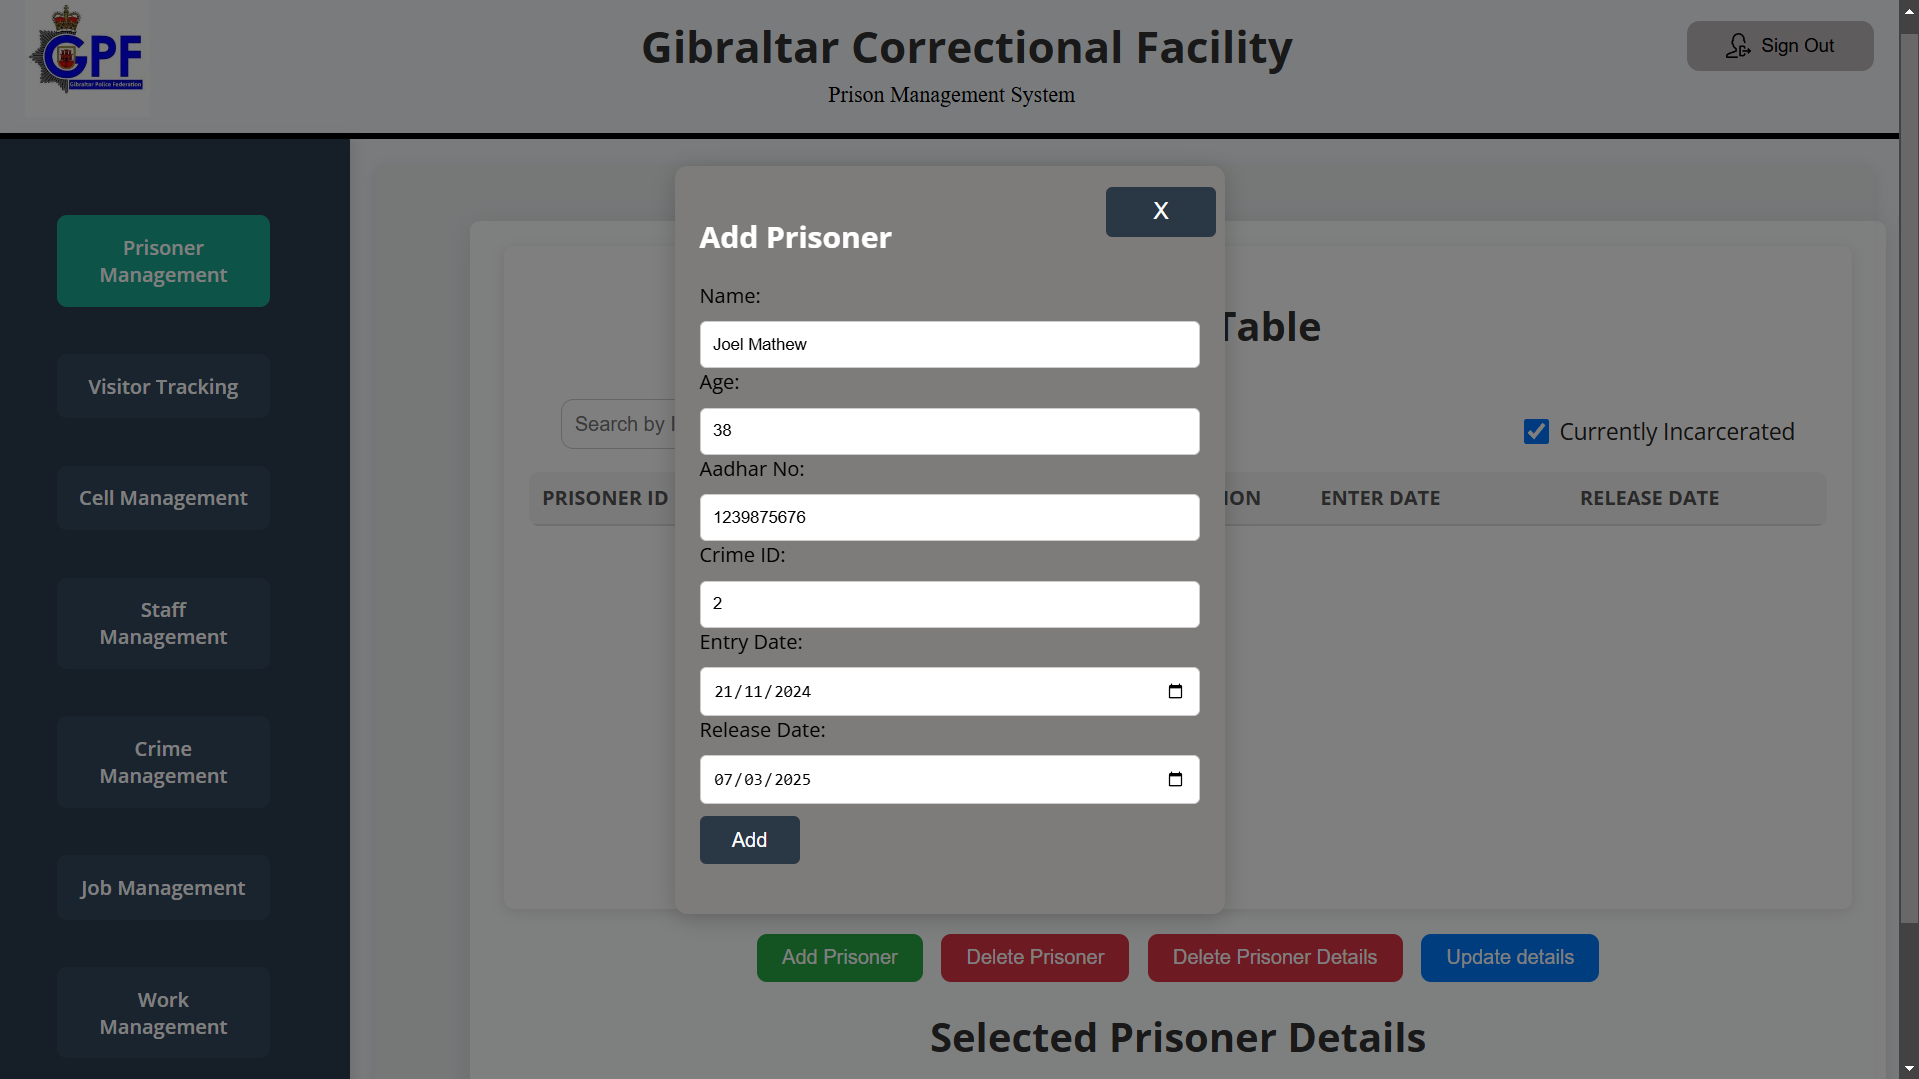
\includegraphics[width=0.8\textwidth]{screenshots/addprisoner.png}
        \caption{Adding a prisoner}
        \label{fig:addp}
    \end{figure}
    \begin{figure}[H]
        \centering
        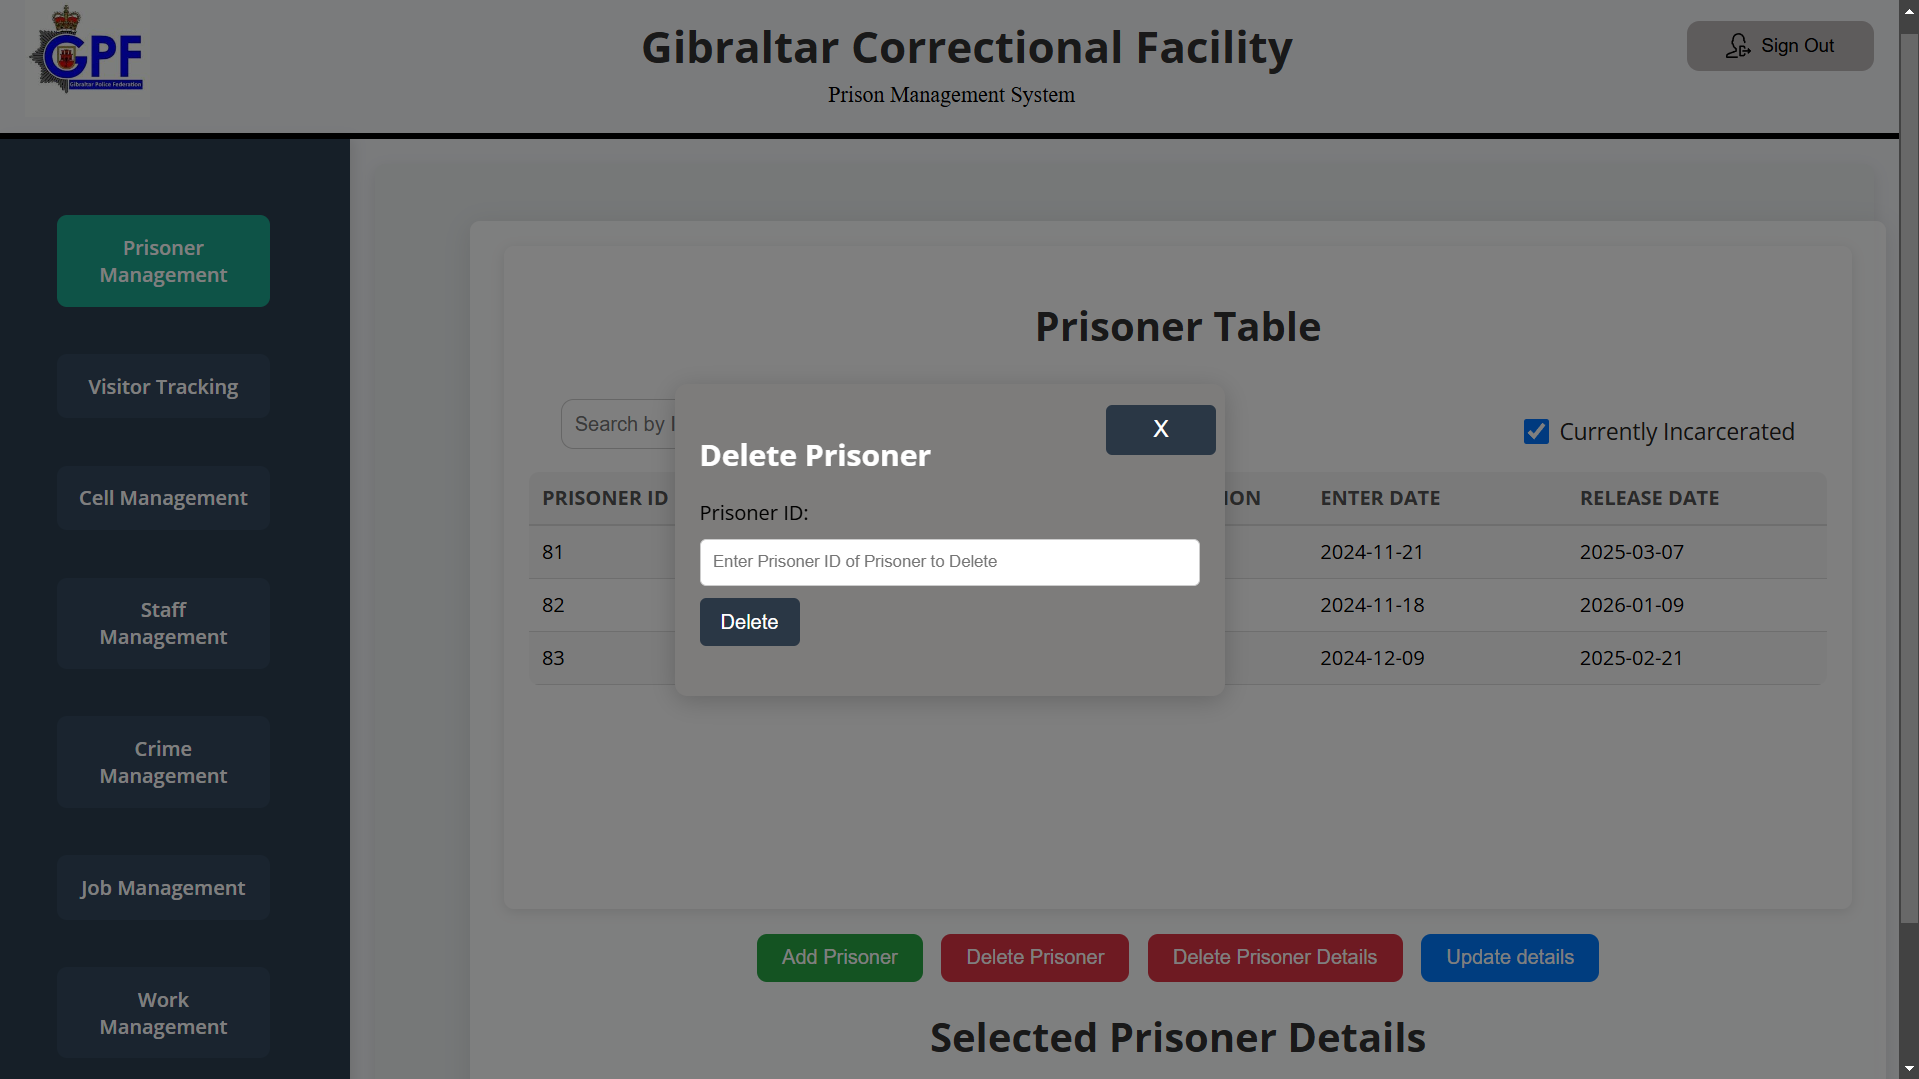
\includegraphics[width=0.8\textwidth]{screenshots/deleteprisoner.png}
        \caption{Deleting a prisoner}
        \label{fig:delprisoner}
    \end{figure}
    \begin{figure}[H]
        \centering
        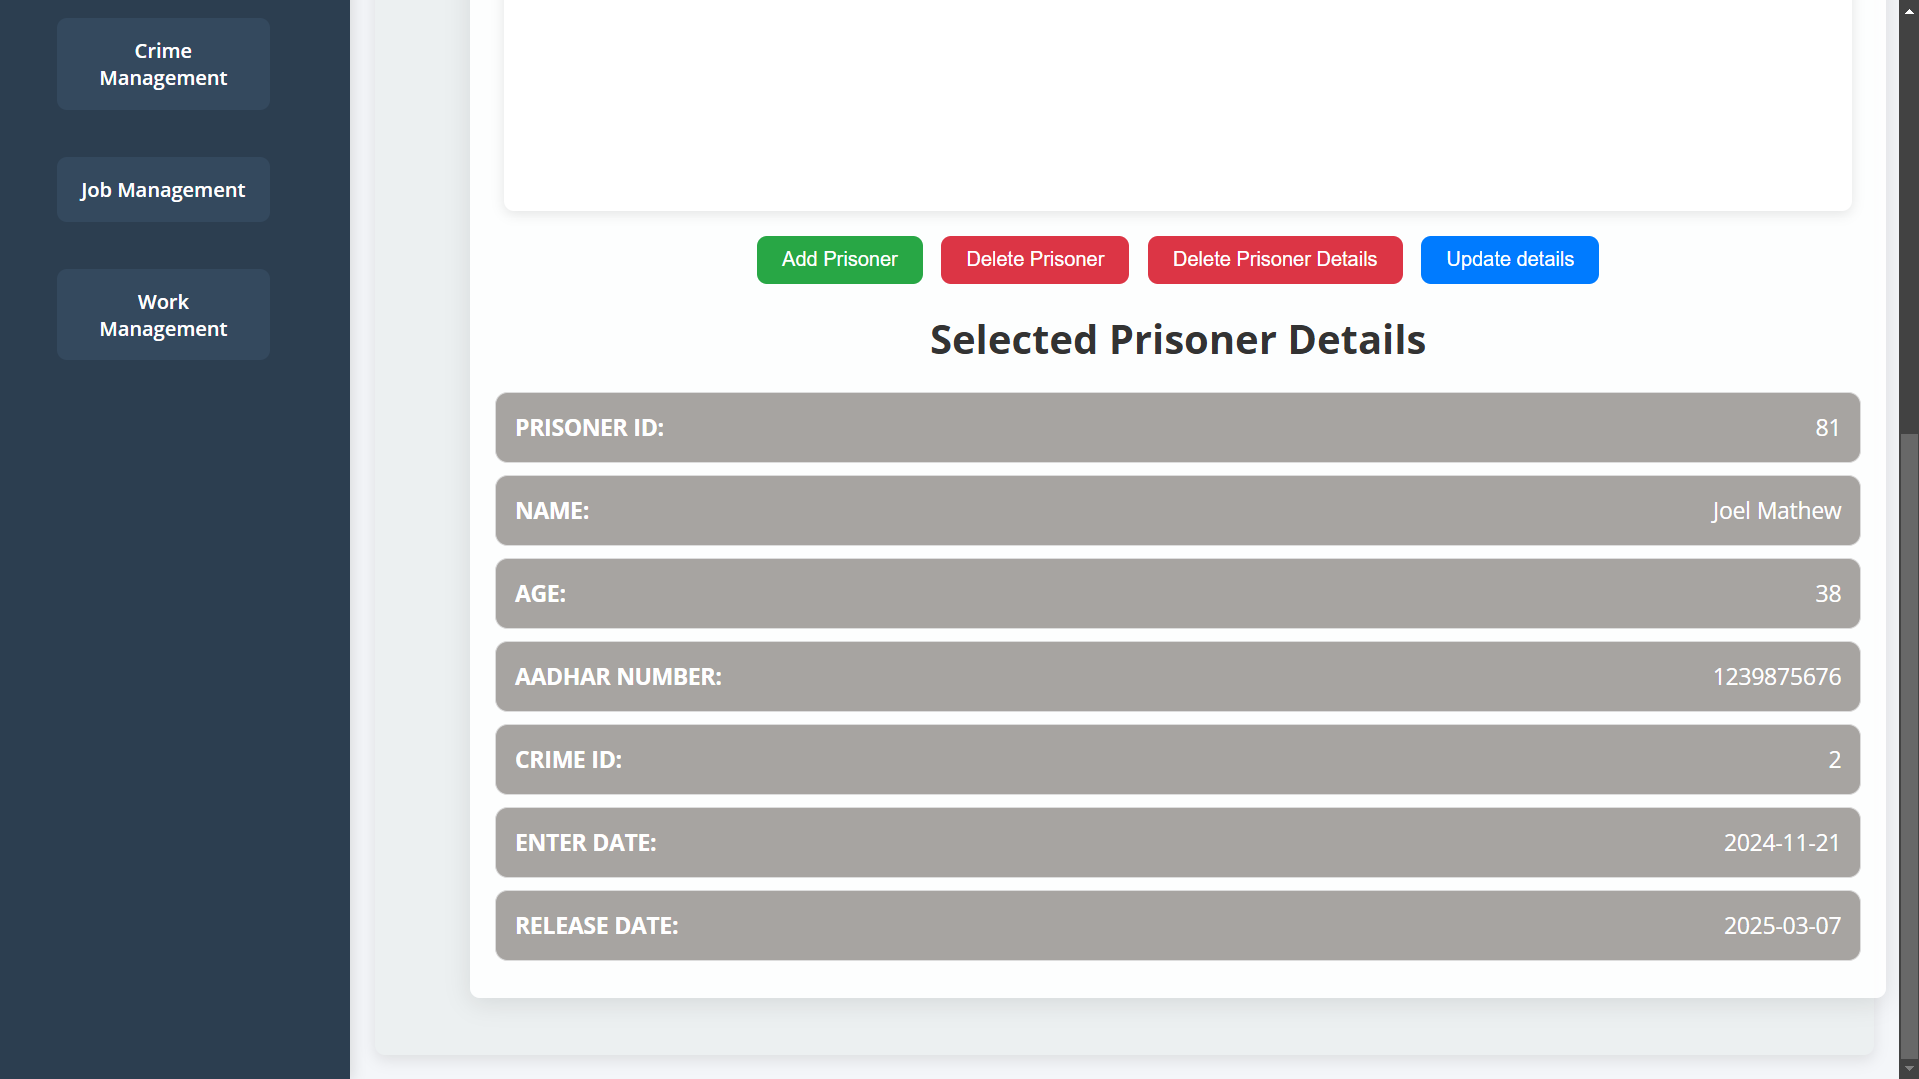
\includegraphics[width=0.8\textwidth]{screenshots/prisonerdetails.png}
        \caption{Viewing a prisoner's details}
        \label{fig:pdet}
    \end{figure}
    \begin{figure}[H]
        \centering
        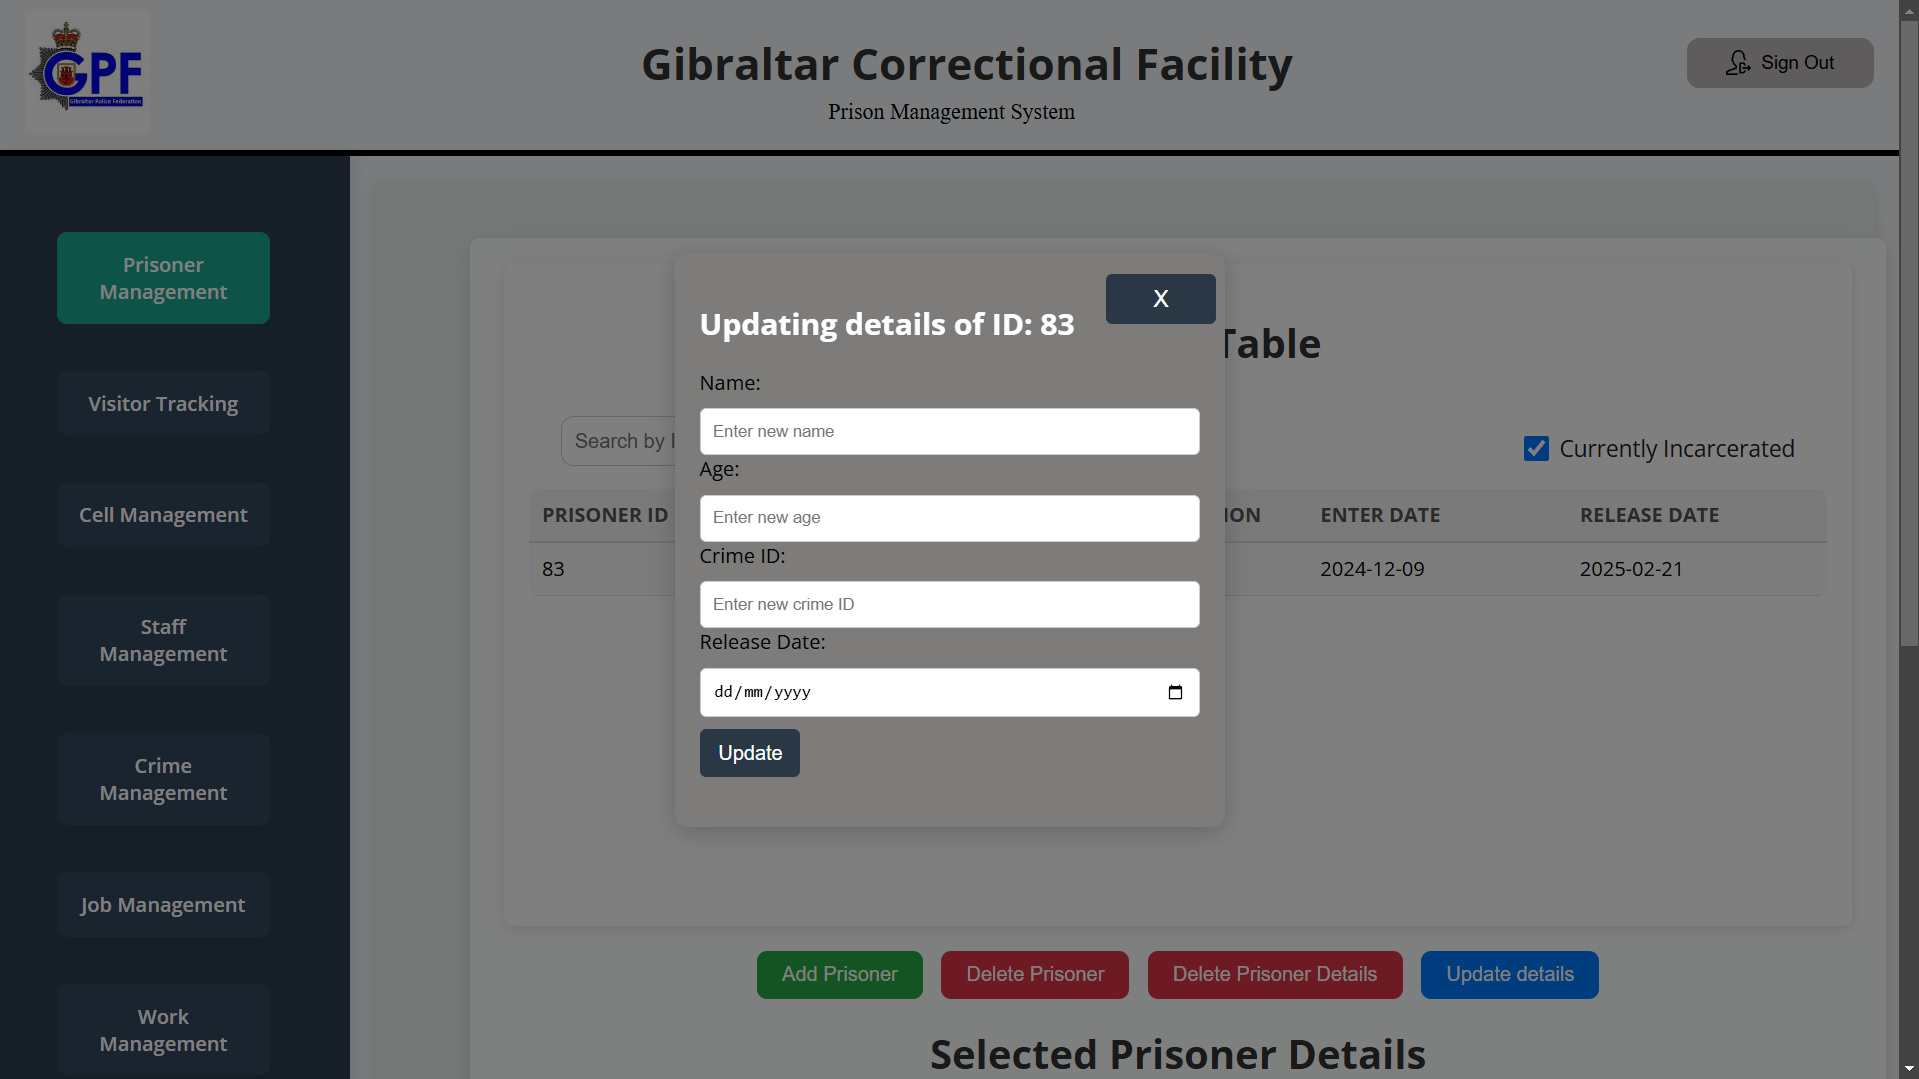
\includegraphics[width=0.8\textwidth]{screenshots/updatedetails.png}
        \caption{Updating a prisoner's details}
        \label{fig:updtp}
    \end{figure}
    \begin{figure}[H]
        \centering
        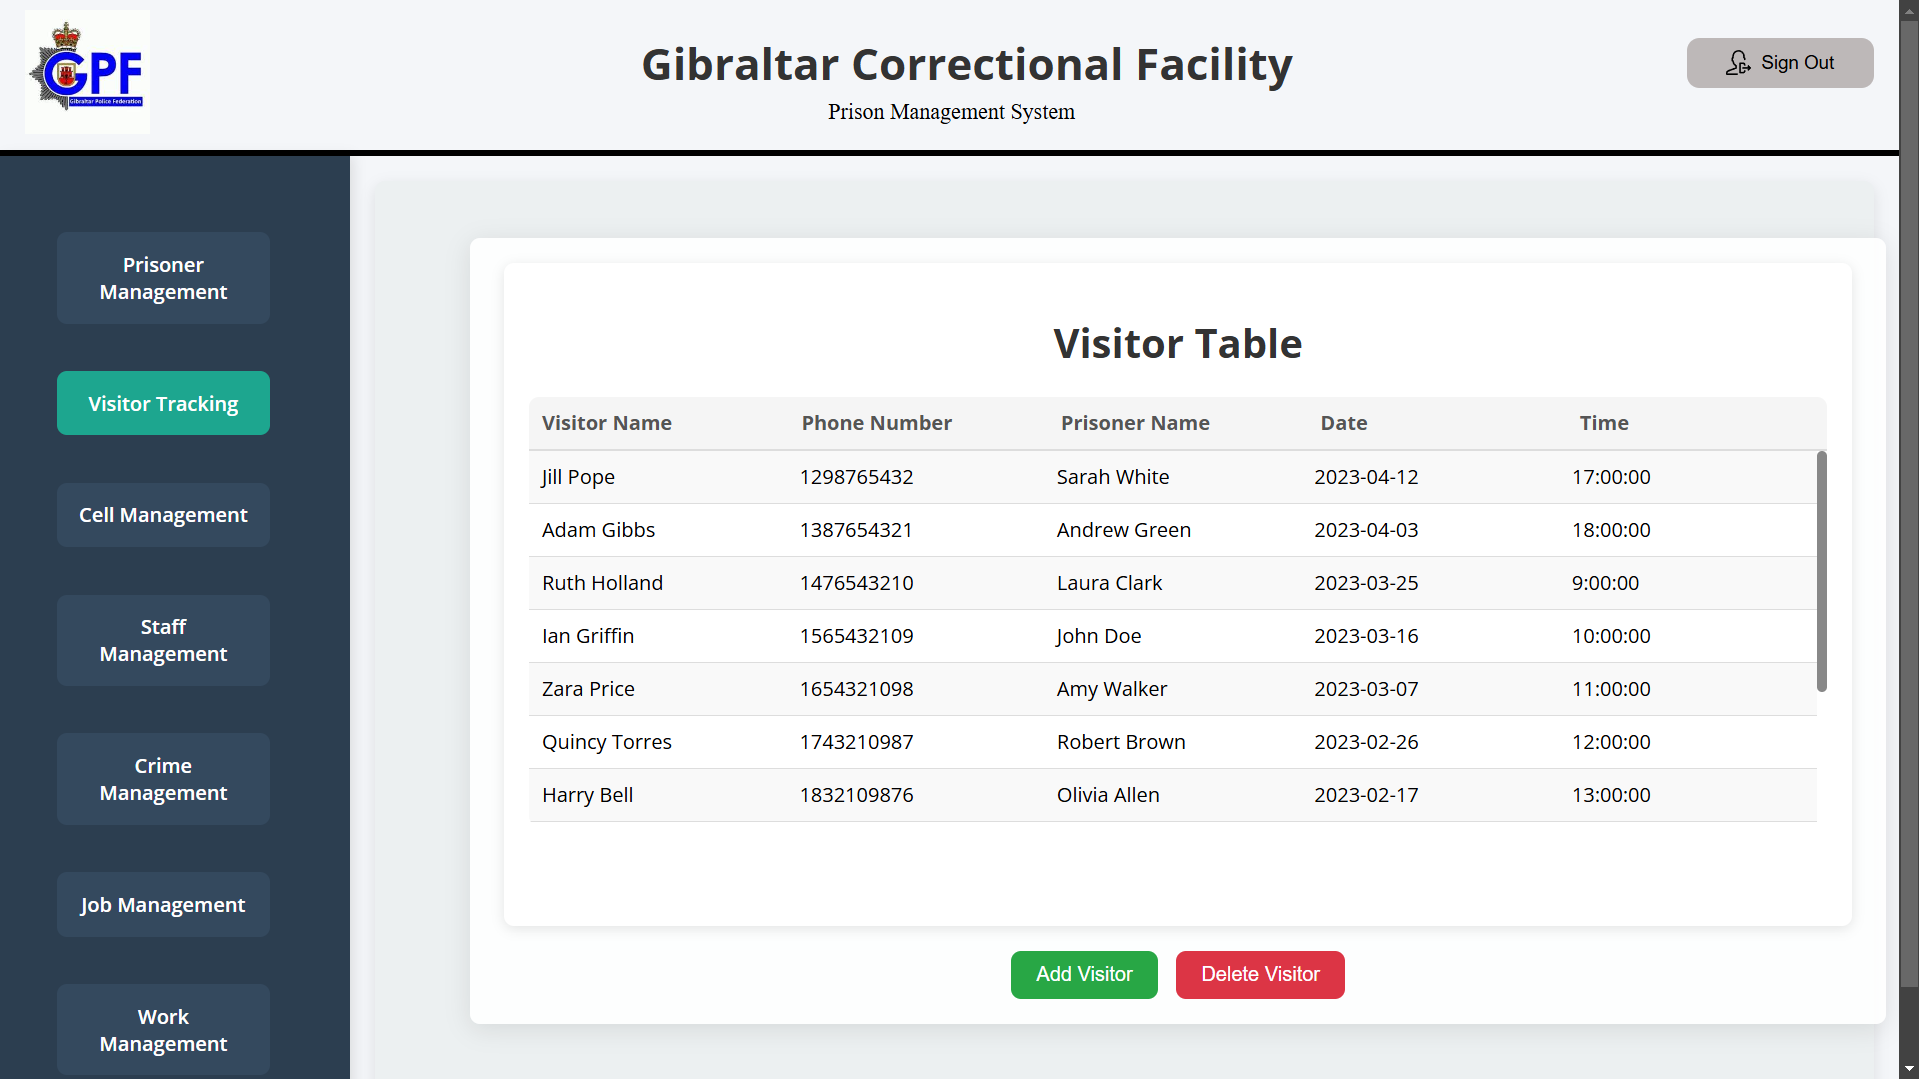
\includegraphics[width=0.8\textwidth]{screenshots/visitor.png}
        \caption{Visitor Tracking}
        \label{fig:visitor}
    \end{figure}
    \begin{figure}[H]
        \centering
        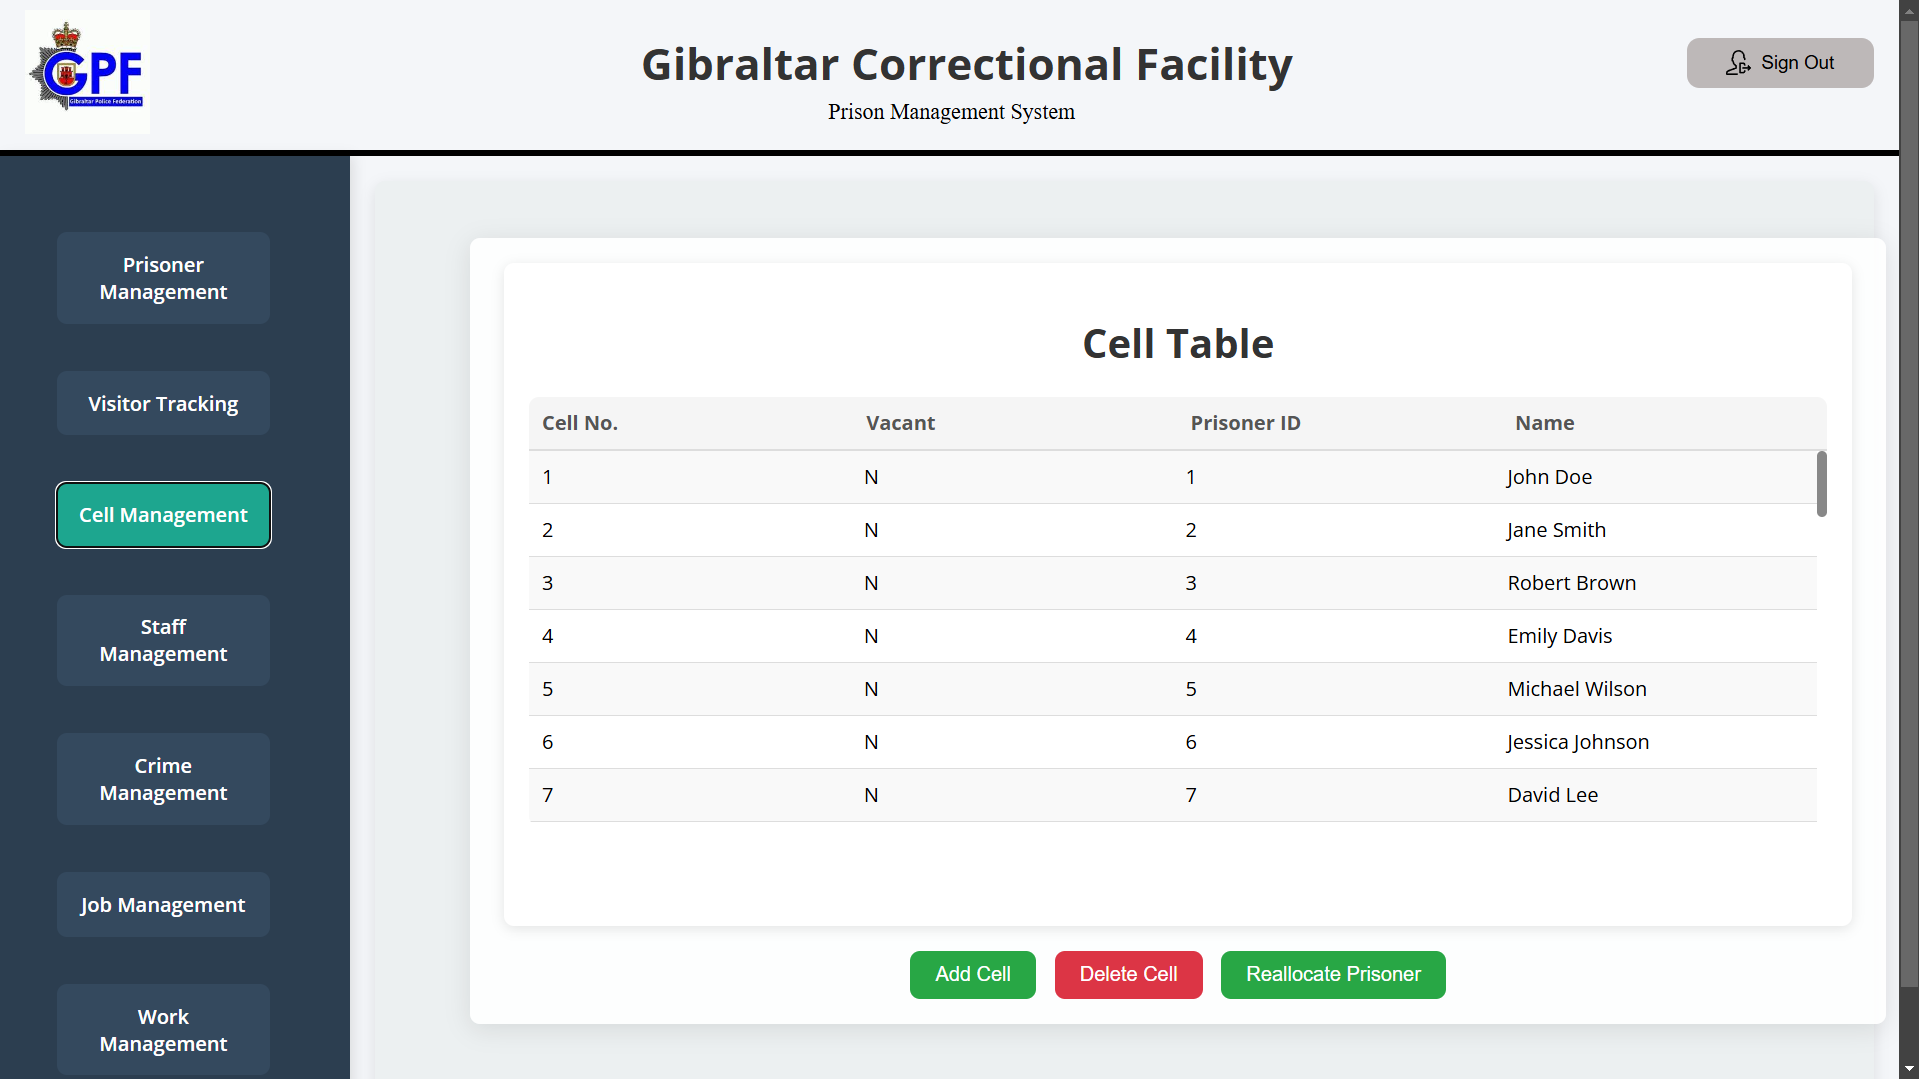
\includegraphics[width=0.8\textwidth]{screenshots/cells.png}
        \caption{Cell Occupants List}
        \label{fig:cells}
    \end{figure}
    \begin{figure}[H]
        \centering
        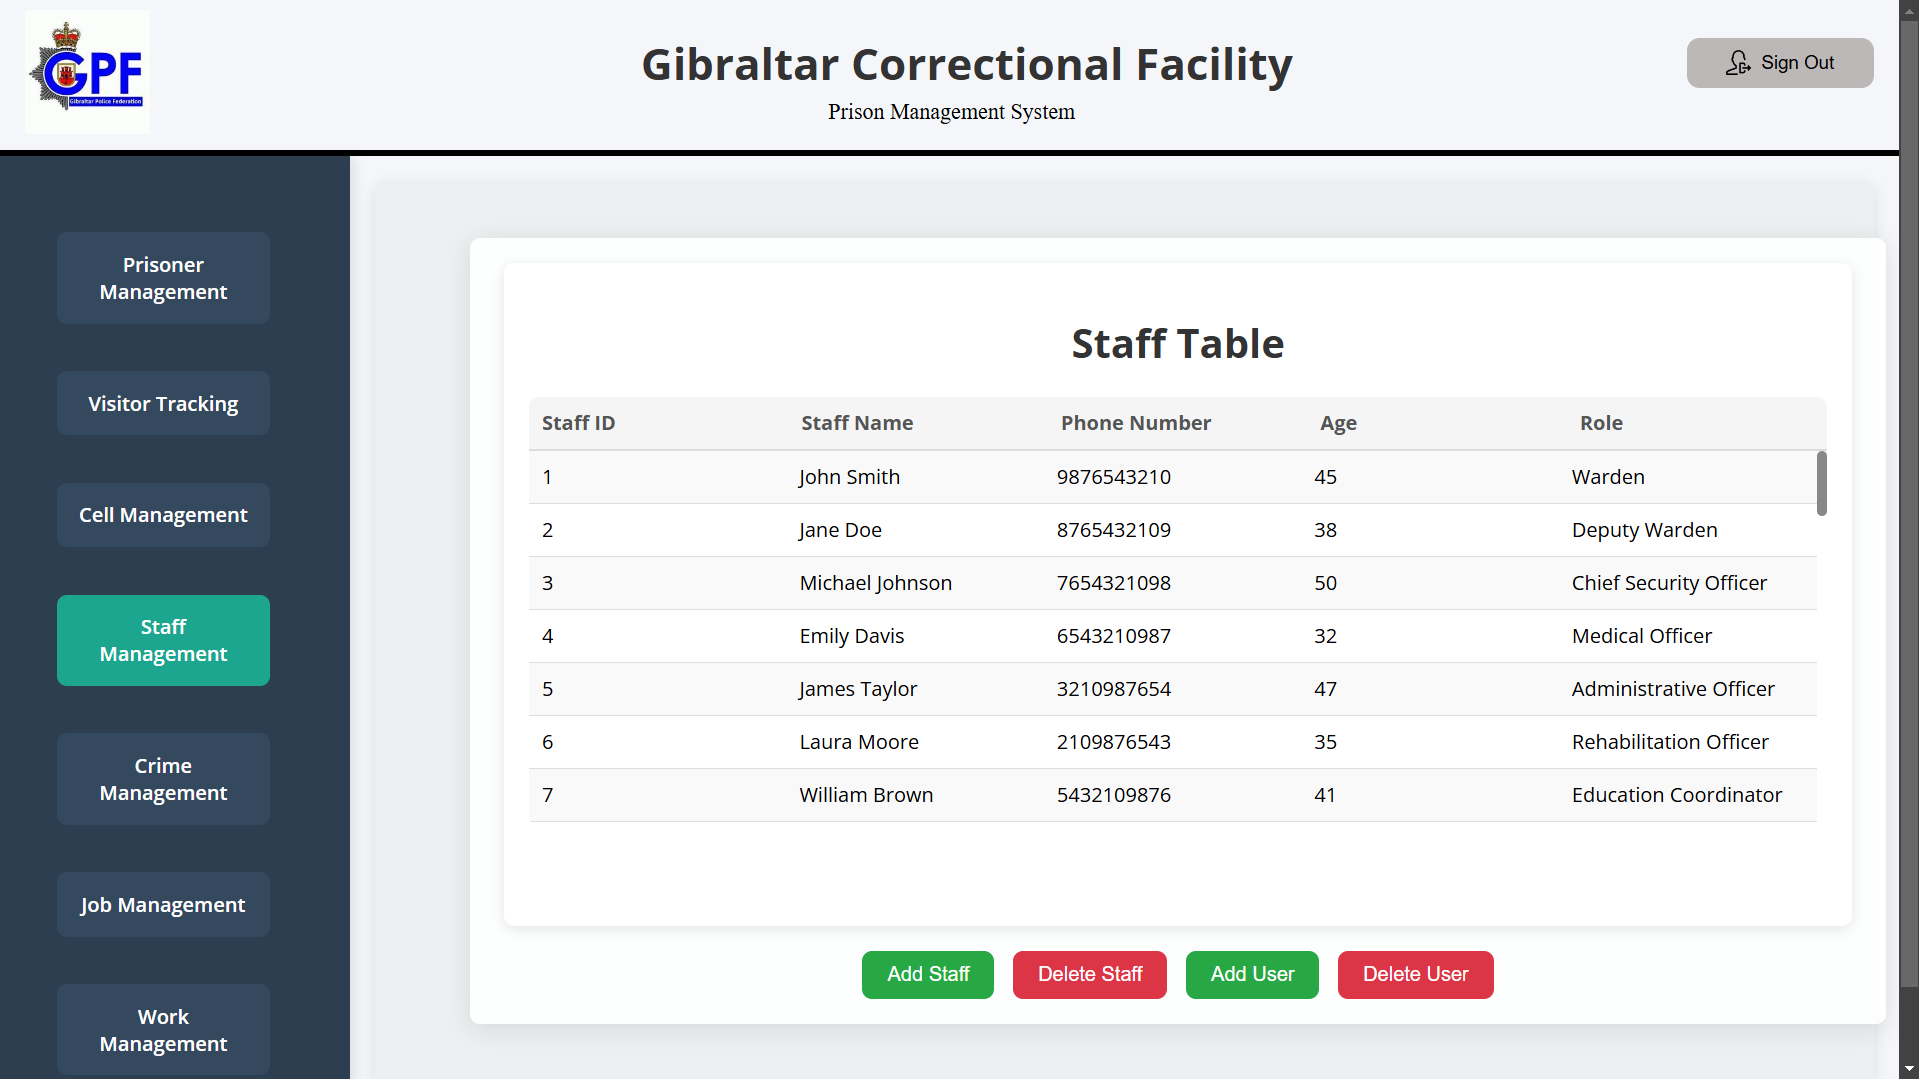
\includegraphics[width=0.8\textwidth]{screenshots/staff.png}
        \caption{Staff Details}
        \label{fig:staff}
    \end{figure}
    \begin{figure}[H]
        \centering
        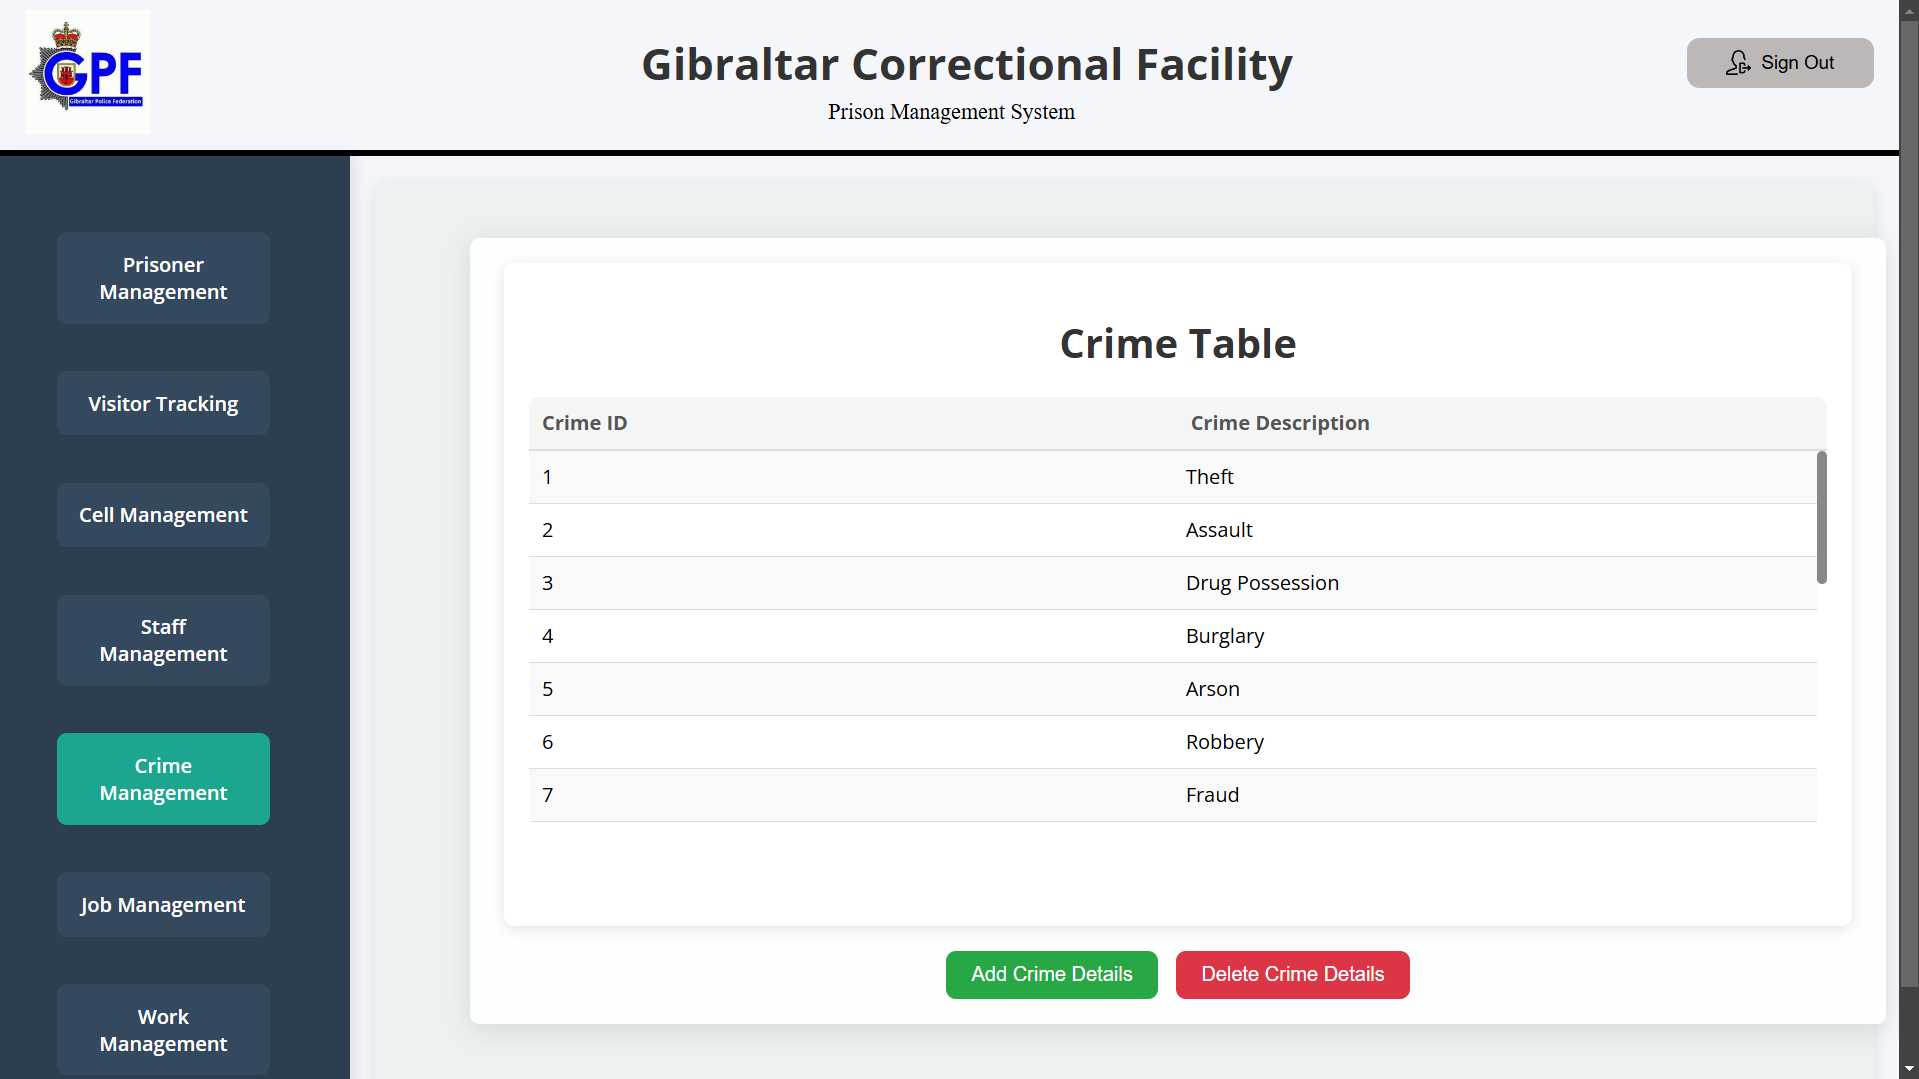
\includegraphics[width=0.8\textwidth]{screenshots/crimes.png}
        \caption{List of Crimes}
        \label{fig:crime}
    \end{figure}
    \begin{figure}[H]
        \centering
        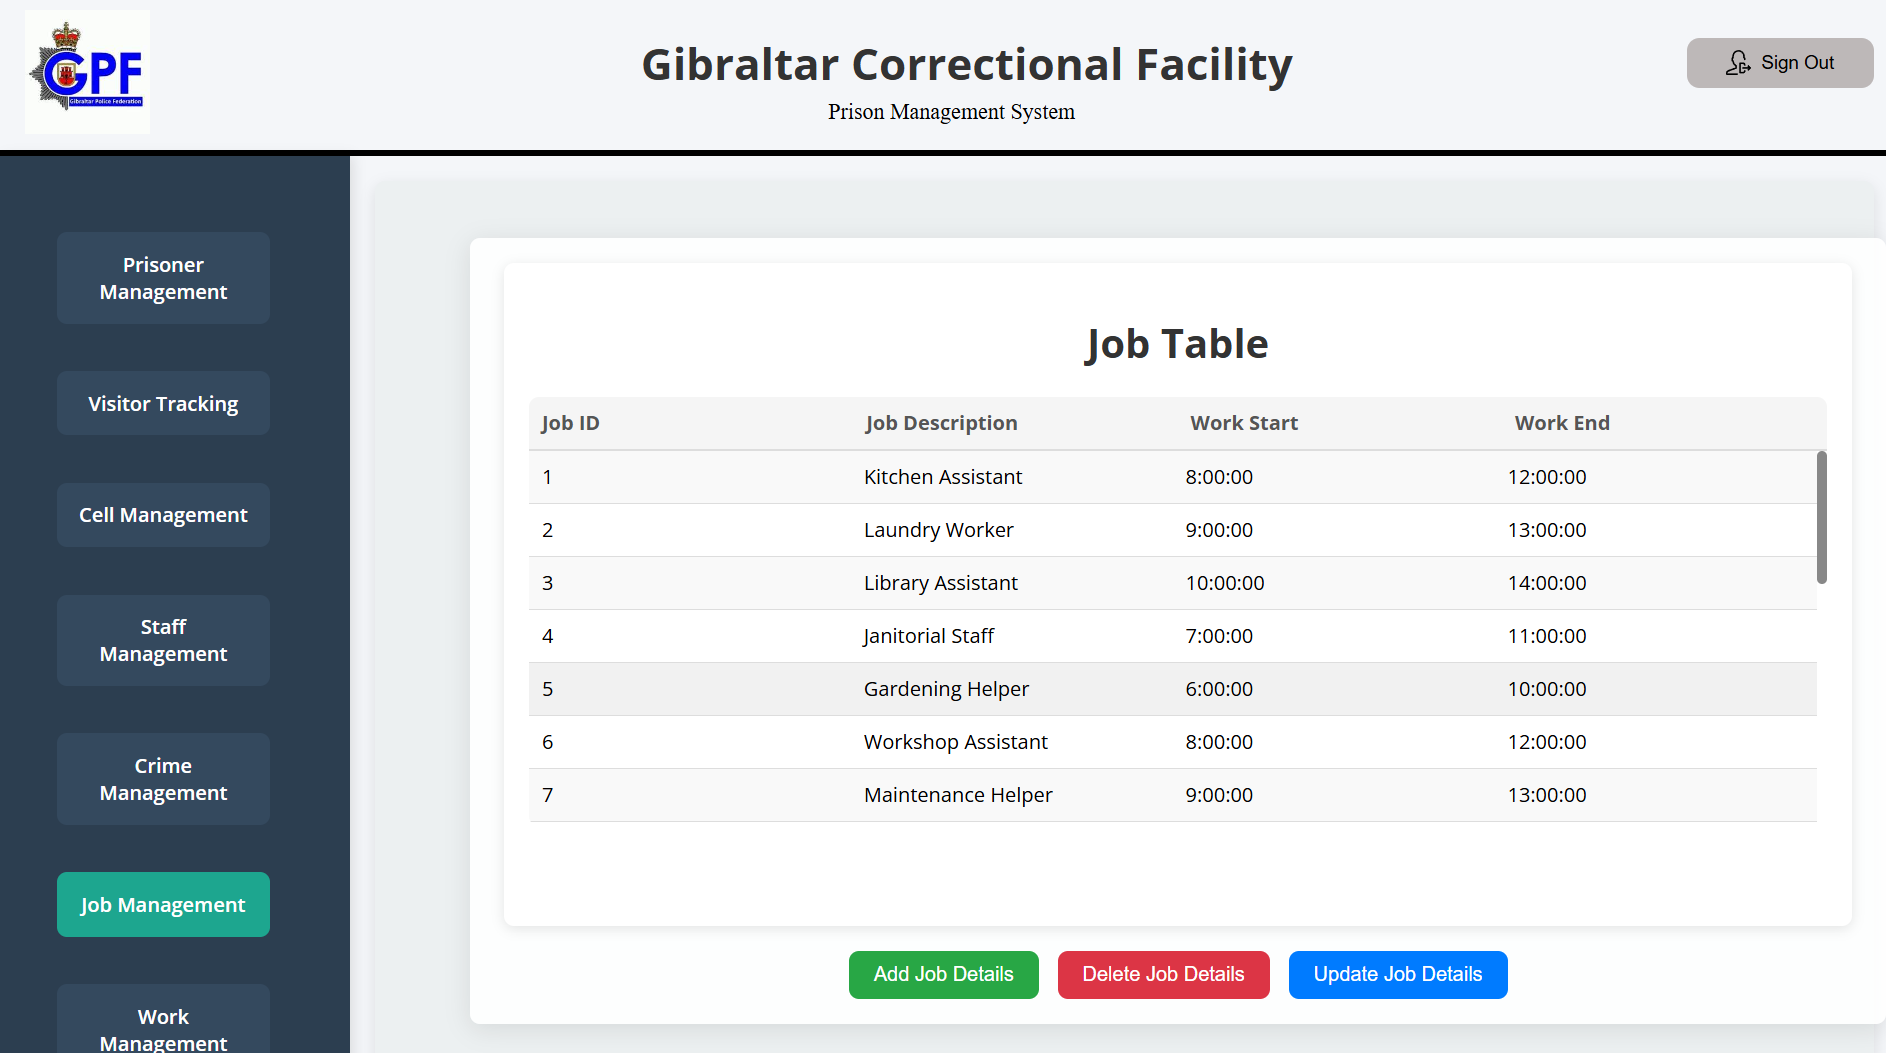
\includegraphics[width=0.8\textwidth]{screenshots/jobs.png}
        \caption{List of jobs available to prisoners}
        \label{fig:jobs}
    \end{figure}
    \begin{figure}[H]
        \centering
        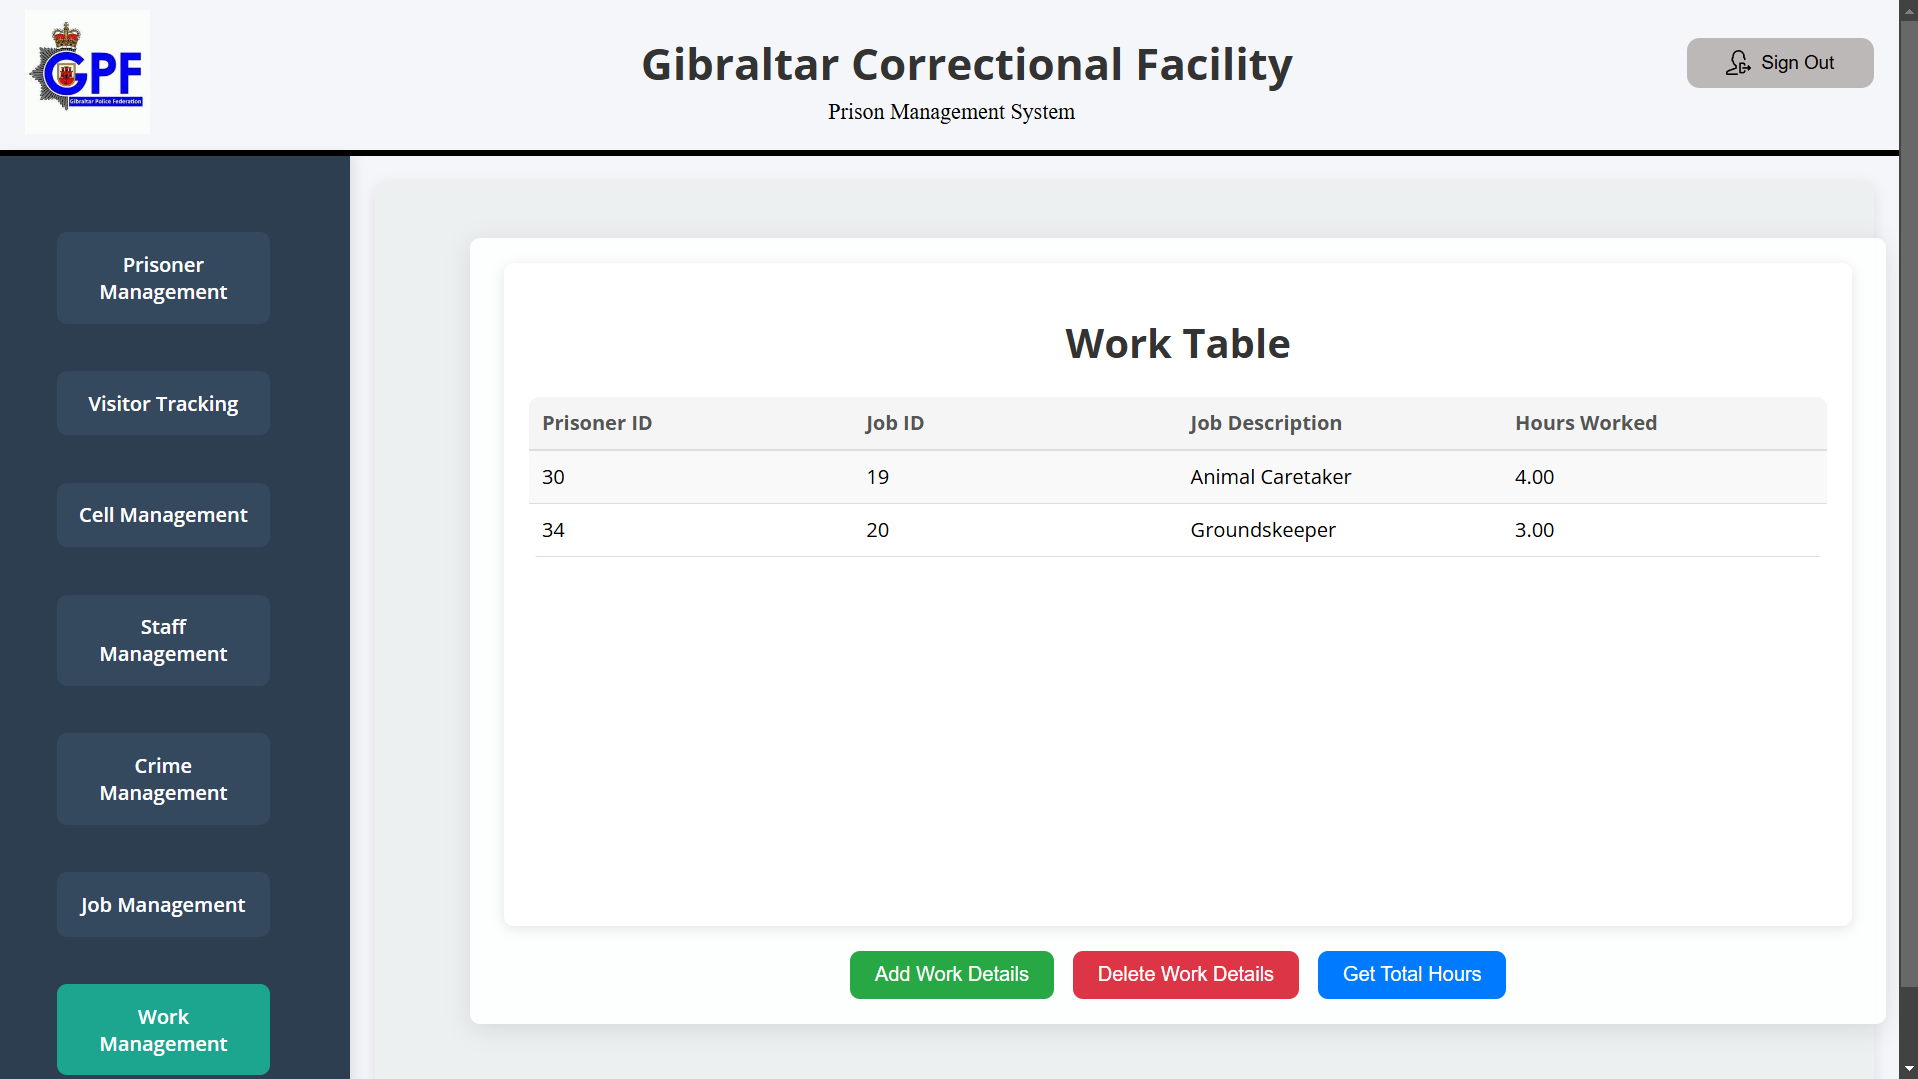
\includegraphics[width=0.8\textwidth]{screenshots/work.png}
        \caption{Details of community service}
        \label{fig:work}
    \end{figure}

\chapter{Conclusion}

The Prison Management System is an effective tool that brings structure and organization to the challenging task of prison administration. It enables secure, efficient and accurate management of all aspects of a prison. This system provides a clear, user-friendly experience that supports daily operations. Staff members can efficiently manage records and quickly access essential information, enhancing workflow and reducing the likelihood of errors. By enabling staff to accurately monitor and keep track of all details regarding a prisoner digitally, the PMS is able to eliminate slow and inaccurate manual record keeping duties. By automating these tedious tasks, the prison staff are able to focus on the safety and security of the prison and its prisoners.
 
The modular design of the system allows it to adapt to different needs and ensures that each task is handled smoothly and securely. Overall, this project demonstrates a thoughtful approach to creating a well-organized, efficient, and secure environment for prison operations.


\chapter{Future Scope}
\section{Advanced Search and Filtering}
\begin{itemize}
    \item \textbf{Filter by Date}: For records such as crimes, work hours, and visits, users could filter data by specific time frames or ranges.
    \item \textbf{Search by Multiple Criteria}: Enable multi-parameter searches, e.g., finding prisoners who are in a specific cell and have a certain job or crime.
\end{itemize}

\section{Automated Notifications and Alerts}
\begin{itemize}
    \item \textbf{Visitor Notifications}: Automatic email or system notifications for visitors and staff, confirming upcoming visits.
    \item \textbf{Cell Reallocation Alerts}: Notification to staff when prisoners are moved between cells or when a new cell is added.
    \item \textbf{Staff/Visitor Monitoring}: Alerts to senior staff when suspicious or unauthorized activities occur, such as when a visitor is added without proper clearance or a prisoner is reallocated inappropriately.
\end{itemize}

\section{Other Enhancements}
\begin{itemize}
    \item \textbf{Parole Tracking}: Add a feature to track parole eligibility and status for prisoners, ensuring that all necessary data and documents are recorded and updated.
    \item \textbf{Rehabilitation History}: Record and track a prisoner’s rehabilitation history, including completed programs, attendance, and progress reports.
\end{itemize}

%%********************References**********
%%****This template uses IEEE bibliography style

 \begin{thebibliography}{99}
    \bibitem{yong2017} Yong, J., \& Liu, X., \emph{A Smart Prison Management System Based on Internet of Things}, \textit{International Journal of Smart Home}, vol. 11, no. 6, pp. 1--10, 2017.

    \bibitem{pennefather2018} Pennefather, S., \& MacFarlane, A., \emph{Automated Prison Management: Bridging the Gap Between Traditional and Modern Security Systems}, \textit{Journal of Criminal Justice}, vol. 55, pp. 45--58, 2018.

    \bibitem{reactdocs} React Team, \emph{React - A JavaScript library for building user interfaces}, \textit{React Documentation}, [Online]. Available: https://reactjs.org/docs/getting-started.html. [Accessed: Nov. 8, 2024].

    \bibitem{flaskdocs} Flask Team, \emph{Flask - A micro web framework written in Python}, \textit{Flask Documentation}, [Online]. Available: https://flask.palletsprojects.com/en/2.2.x/. [Accessed: Nov. 8, 2024].
\end{thebibliography}

\end{document}